\documentclass[11pt]{article}

\usepackage[a4paper,margin=2.5cm]{geometry}
\usepackage{graphicx}
\graphicspath{{figures/}}
\usepackage{amsmath,amssymb,amsthm}
\usepackage{mathrsfs}
\usepackage[colorlinks=true,linkcolor=blue,citecolor=blue,urlcolor=blue]{hyperref}
\usepackage{booktabs}
\usepackage{enumitem}
\usepackage{natbib}

\theoremstyle{plain}
\newtheorem{theorem}{Theorem}[section]
\newtheorem{conditional}[theorem]{Conditional Proposition}
\newtheorem{proposition}[theorem]{Proposition}
\newtheorem{corollary}[theorem]{Corollary}
\newtheorem{lemma}[theorem]{Lemma}
\theoremstyle{definition}
\newtheorem{definition}[theorem]{Definition}
\newtheorem{axiom}[theorem]{Axiom}
\newtheorem{hypothesis}[theorem]{Hypothesis}
\newtheorem{interpretation}[theorem]{Interpretation}
\theoremstyle{remark}
\newtheorem{remark}[theorem]{Remark}

\newcommand{\Zphi}{\mathbb{Z}[\varphi]}
\newcommand{\Fix}{\mathrm{Fix}}
\newcommand{\Ical}{\mathcal{I}}
\newcommand{\Ocal}{\mathcal{O}}
\newcommand{\Ccal}{\mathcal{C}}
\newcommand{\Mcal}{\mathcal{M}}
\newcommand{\Acal}{\mathcal{A}}
\newcommand{\Bcal}{\mathcal{B}}
\newcommand{\Rcal}{\mathcal{R}}
\newcommand{\Dcal}{\mathcal{D}}
\newcommand{\Pcal}{\mathcal{P}}
\newcommand{\Xcal}{\mathcal{X}}
\newcommand{\Cph}{C_\varphi}
\newcommand{\Ilife}{\Ical_{\mathrm{life}}}

\title{Life as Closure\\[6pt]
\large Agency, Meaning, and the Mechanics of Individual Purpose}
\author{%
  Lee Smart\\[4pt]
  \textit{Institute of Vibrational Field Dynamics}\\[2pt]
  \texttt{contact@vibrationalfielddynamics.org}\\[2pt]
  \texttt{@vfd\_org}%
}
\date{May 2026}

\begin{document}

\maketitle

\noindent\textbf{Status:} Preprint (not peer-reviewed). Human-facing flagship companion to \citet{SmartExistenceClosure}. The core paper supplies the formal closure machinery: distinction, relation, closure operator, symmetry, bounded reference frames, per-frame zero-lines, embedding into universal structure. The present paper applies that machinery to living systems. It asks what closure means \emph{when localised} as boundary, repair, memory, action, relevance, agency, and relation; and gives the structural objects that supply these. The contribution is mechanical, not metaphorical: each notion is supplied with a formal definition, a quantitative measure, and a falsifier. The phenomenological reading is conditional on the Access Principle (P-A); the structural definitions are formal. Two technical companions extend the same machinery into neuroscience (\citet{SmartProcessingToPOV}) and cosmology (\citet{SmartCosmicClosure}). The present paper is the human bridge.

\begin{abstract}
A living system is a bounded reference frame that must persist on a substrate exposed to perturbation. We propose a single structural account: a living frame is the data $\Ilife = (\Ocal, \Ccal_\Ocal, \Bcal, \Mcal, \Acal, \Sigma_\Ical)$, where $\Ocal$ is the substrate, $\Ccal_\Ocal$ the self-referential constraint, $\Bcal$ the boundary, $\Mcal$ the memory, $\Acal$ the action policy, and $\Sigma_\Ical \subseteq \Fix(\tau)$ the per-frame zero-line, all defined on the closure-operator machinery of \citet{SmartExistenceClosure}. The contribution is that this single object generates operator-level mechanics for the human-experience phenomena typically treated separately: relevance, dyscoherence, agency, purpose, joint meaning, emotions, thoughts, identity through time, trauma and its healing, flow, creativity, hope and despair, trust, self-deception, and (under the Access Principle) qualia. Each is a derived structural object with a formal definition, a stated falsifier, and a numerical demonstration on the $V_{600}$ substrate (L1--L13 in \texttt{repro/life\_demo.py}, deterministic at seed 42). The empirical anchor is the cortical phase closure data of \citet{SolutionLab002}: 14/14 propofol subjects positive ($t = 7.11$, $d_z = 1.90$, $p < 2 \times 10^{-4}$), source-localised replication 14/14 ($t = 9.72$), cross-cohort replication 7/7 clinical anaesthesia; the cross-substrate methodology of \citet{SmartClosureDistance} further validates the anchor with leave-one-subject-out feature-reselection ($d_z = 2.07$, Jaccard $= 1.00$, two-feature minimal closure: beta-PGD plus alpha:beta cross-band PLV), an \emph{a priori} applicability diagnostic, and an overall classification record of $15$ of $16$ tested cases matching observed PASS/FAIL across paired-design substrates plus four post-draft real-data EEG cohorts (trait anxiety $d = +0.79$ predicted-PASS-leaning / observed-PASS, musical hyperscanning $d_z = +0.23$ predicted-FAIL / observed-FAIL, Alzheimer's disease $d = -0.31$ predicted-FAIL / observed-FAIL, frontotemporal dementia $d = +0.02$ predicted-PASS / observed-FAIL --- one transparently characterised false positive attributable to a directional-cancellation limitation of the current unpaired-design thresholds). The dementia results in particular scope the framework: closure-as-distance tracks \emph{functional} integration of an intact integrative network (anaesthesia, anxiety), not loss of integration through structural neurodegenerative atrophy. The life-paper claim is therefore: living systems require the functional integrative organisation that closure measures; structural neurodegenerative loss is a distinct phenomenon needing methodology adapted to feature-asymmetric cancellation patterns. The discipline throughout is \emph{mechanics, not meaning}: the framework supplies operator-level structural objects that carry each notion, with stated falsifiers; it does not legislate the phenomenology those mechanics may underwrite. The Access Principle is named as an open conjecture, not asserted.
\end{abstract}
\paragraph{Programme map (review-packet 2026-05-22).}
This paper is part of the Existence / Life / Closure review packet. Stable packet references:
Paper I = \emph{Existence as Closure};
Paper II = \emph{Life as Closure};
Paper III = \emph{From Processing to Point of View};
Note A = \emph{Bioelectric Closure} (SL-001);
Note B = \emph{Cortical Phase Closure} (SL-002);
Note C = \emph{Closure-as-Distance} (cross-substrate methodology);
Note D = \emph{Trauma / Cortical Closure} (SL-005);
Note E = \emph{FlowIndex} (SL-006);
Note F = \emph{Dyadic Joint Meaning} (SL-007).
Extension IV = \emph{Cosmic Self-Pruning and Frame Recurrence} is withheld from the primary packet.

\paragraph{Status taxonomy.}
\textbf{Theorem / Definition} = formal structural claim under stated assumptions.
\textbf{Conditional Proposition} = bridge claim depending on H-RP, P-A, substrate mapping, or empirical interpretation.
\textbf{Empirical Result} = completed data analysis with stated effect size + significance.
\textbf{Empirical Proxy} = measurable first-order approximation, not the formal operator.
\textbf{Pre-registered Proposal} = future test, not evidence.



%==================================================================
\section{Introduction}\label{sec:intro}
%==================================================================

\subsection{Position relative to the foundation}

The companion paper \citet{SmartExistenceClosure} answers: \emph{what is existence, structurally?} Its answer is the existence-as-closure principle:
\[
  X \text{ is admissible} \quad\Longleftrightarrow\quad \Ccal(X) = X \text{ and } \tau(X) = X.
\]
Within that paper's framework, a bounded reference frame $\Ical = (\Ocal, \Ccal_\Ocal, p, \Lambda, t_0)$ is the local realisation of this principle: a finite projection of the universal closure structure with a self-referential constraint. The frame admits a per-frame zero-line $\Sigma_\Ical \subseteq \Fix(\tau)$ of computable dimension, the dimension being the frame's structural complexity. Local frames embed into the universal closure structure via an explicit projection $!_\Ical(v) = \pi_\Ical(P_{\Sigma_\Ical}(v))$.

The present paper asks the next question: \emph{what does that closure structure become when localised as life?} A planarian, a person, a culture, a conversation, an ecosystem --- each is a candidate bounded reference frame. But none is just a frame: each maintains a self/world boundary, repairs damage, carries memory across closure ticks, selects action, distinguishes the relevant from the irrelevant, and forms joint frames with others. These are not arbitrary features. They are the operational consequences of being a bounded reference frame that must persist on a substrate exposed to perturbation.

This paper supplies the structural objects.

\subsection{What this paper is}

This paper builds eighteen structural objects on top of the bounded reference frame, in three layers:

\textbf{Eight primitive objects on the living frame:}
\begin{enumerate}[leftmargin=2em]
\item The \textbf{living-frame definition} $\Ilife = (\Ocal, \Ccal_\Ocal, \Bcal, \Mcal, \Acal, \Sigma_\Ical)$ (\S\ref{sec:living-frame}).
\item The \textbf{boundary} $\Bcal = (\partial \Ocal, \Phi_\Bcal)$ and the boundary-maintenance conditional proposition (\S\ref{sec:boundary}).
\item The \textbf{repair dynamic} with characteristic time $\sim 1/(\lambda \mu)$ closure ticks (\S\ref{sec:repair}).
\item The \textbf{memory} $\Mcal = (\mathsf{Store}, \mathsf{Write}, \mathsf{Read})$ on a closure-stable subspace of $\Sigma_\Ical$ (\S\ref{sec:memory}).
\item The \textbf{action policy} $\Acal$ and \textbf{agency gradient} $a^* = \arg\max_a \mathbb{E}[\Delta\Ccal \mid a]$ (\S\ref{sec:action}).
\item The \textbf{relevance function} $\Rcal_\Ical(x) = |\dim\Sigma(t+\Delta t \mid x) - \dim\Sigma(t+\Delta t \mid \neg x)|$ (\S\ref{sec:relevance}).
\item The \textbf{dyscoherence measure} $\Dcal_\Ical(v) = \|v - P_{\Sigma_\Ical}(v)\|$ as bounded proxy for suffering (\S\ref{sec:dyscoherence}).
\item The \textbf{purpose} $\Pcal(\Ilife)$ as time-integrated agency, and the \textbf{joint-meaning quantity} $\delta_{AB}$ for frames in relation (\S\S\ref{sec:purpose}, \ref{sec:joint-meaning}).
\end{enumerate}

\textbf{Three mental-state objects} (\S\S\ref{sec:emotions}, \ref{sec:thoughts}, \ref{sec:phenomenology}):
\begin{enumerate}[leftmargin=2em, start=9]
\item The \textbf{emotional state} $\mathbf{e}_\Ical(t)$ as an activation vector across a closure-stable eigenmode decomposition of $\Sigma_\Ical$ --- mechanics of emotion, not meaning.
\item The \textbf{thought trajectory} $\gamma$ as a closure-tick path through $\Sigma_\Ical$ --- mechanics of cognition, not content.
\item The \textbf{spectral signature} $\mathbf{s}_\Ical(F_t)$ as conditional correlate of qualitative character under P-A.
\end{enumerate}

\textbf{Seven further structural objects} obtained by composing the primitives (\S\ref{sec:further-objects}):
\begin{enumerate}[leftmargin=2em, start=12]
\item \textbf{Identity across time} as preserved closure-pattern continuity, not preserved substrate (\S\ref{sec:identity}).
\item \textbf{Trauma and healing} as closure-stable memory pattern + access-reweighting therapy (\S\ref{sec:trauma}).
\item \textbf{Flow} as simultaneous satisfaction of four structural conditions, with time-dilation as conditional proposition (\S\ref{sec:flow}).
\item \textbf{Creativity} as trajectory whose content support escapes $\mathsf{Read}_\Mcal(\mathsf{Store}_\Mcal)$ (\S\ref{sec:creativity}).
\item \textbf{Hope and despair} as forward temporal projection of expected purpose (\S\ref{sec:hope-despair}).
\item \textbf{Trust} as sustained joint-frame compatibility $\kappa_{AB}$ under perturbation (\S\ref{sec:trust}).
\item \textbf{Self-deception} as closure-stable belief sustained by boundary filtering (\S\ref{sec:self-deception}).
\end{enumerate}

Each is a formal definition with a quantitative measure, a stated falsifier, and a numerical demonstration (L1--L13) in the sim suite \texttt{repro/life\_demo.py}. The operator-level definitions are formal; the phenomenological readings --- what redness, anger, or insight feel like --- are P-A-conditional and named as such throughout. The framework supplies the mechanics; it does not legislate what those mechanics mean.

\subsection{What this paper is not}

\begin{itemize}[leftmargin=2em]
\item Not a re-derivation of the closure framework. Theorems on $\Cph$, $\tau$, $\Sigma_\Ical$, and $!_\Ical$ are imported from \citet{SmartExistenceClosure}; this paper applies them.
\item Not a theological or metaphysical claim. The framework's commitments are operator-level: $\Bcal$, $\Mcal$, $\Acal$ are mathematical objects, not spiritual ones. Phenomenological readings (``meaning,'' ``purpose,'' ``suffering'') are explicitly conditional on the Access Principle (P-A) and named as conjectural.
\item Not a reduction of suffering to a number. $\Dcal_\Ical$ is a structural distance, supplied as a proxy. The framework does not claim that minimising $\Dcal_\Ical$ exhausts what it is to alleviate suffering; it claims that $\Dcal_\Ical$ is the structural component that closure analysis makes visible.
\item Not a manual for how to live. The agency gradient $a^*$ is a structural definition of which actions preserve closure; whether any specific agent should pursue it is a normative question outside the framework.
\item Not a claim that all life is like human life. The living-frame definition applies wherever a bounded reference frame maintains boundary, memory, and action; planarians, cells, ecosystems, and conversations are all candidates at different scales.
\end{itemize}

\subsection{Reader's map}

Three commitment levels are available:

\begin{itemize}[leftmargin=2em]
\item \textbf{The living-frame definition} (\S\S\ref{sec:living-frame}--\ref{sec:memory}). The structural extension of $\Ical$ with boundary, repair, and memory. Independent of any specific physical substrate.
\item \textbf{The mechanical objects} (\S\S\ref{sec:relevance}--\ref{sec:joint-meaning}). Relevance, dyscoherence, agency, purpose, joint meaning --- each with a formal definition and a stated quantitative measure.
\item \textbf{The phenomenological bridge} (\S\ref{sec:phenomenology}). The conditional identifications under the Access Principle: relevance as salience, dyscoherence as suffering, agency as choice, purpose as direction, joint meaning as relation.
\end{itemize}

A reader who finds the living-frame definition compelling but rejects the Access Principle reads a mechanical account of living systems without phenomenology. A reader who accepts the Access Principle reads, additionally, a structural account of why those mechanics constitute meaning. The framework is intentionally layered.

\subsection{Central claim: a mechanics of meaning-generation}\label{sec:central-claim}

This paper does not propose a universal content of meaning. It proposes
a universal \emph{mechanics of meaning-generation}. An event, relation,
memory, or action is meaningful to a living frame to the extent that it
changes that frame's future closure capacity. Meaning is therefore
neither arbitrary nor externally imposed; it is generated by the
interaction between boundary, memory, agency, relation, and the frame's
zero-line $\Sigma_\Ical$.

Operationally: if an event $x$ leaves $\dim \Sigma_\Ical(t + \Delta t)$
unchanged conditional on $x$ vs $\neg x$, the framework predicts $x$ is
not meaningful to the frame; the relevance $\Rcal_\Ical(x)$ is the
quantitative measure of this. Joint meaning between two frames is the
generative excess $\delta_{AB}$ on the joint substrate.

The framework's commitment is therefore structural, not normative: the
mechanics by which meaning is generated and measured is the contribution.
What meaning a specific living system finds meaningful in its
specific environment is a separate question --- one the framework
illuminates but does not answer. This distinction is preserved
throughout the paper.

%==================================================================
\section{The living-frame definition}\label{sec:living-frame}
%==================================================================

The bounded reference frame of \citet{SmartExistenceClosure} carries the data
\[
  \Ical = (\Ocal, \Ccal_\Ocal, p, \Lambda, t_0),
\]
with $\Ocal$ a finite vertex set, $\Ccal_\Ocal$ a self-referential constraint, and $(p, \Lambda, t_0)$ an anchor. This is sufficient for a stable bounded reference frame. It is not sufficient for a \emph{living} frame, which must additionally distinguish self from world, carry memory, and act on its environment.

\begin{definition}[Living frame]\label{def:living-frame}
A \emph{living frame} is the data
\[
  \Ilife = (\Ocal, \Ccal_\Ocal, \Bcal, \Mcal, \Acal, \Sigma_\Ical),
\]
where:
\begin{itemize}[leftmargin=2em]
\item $\Ocal$ is the frame's substrate (the finite vertex set of the underlying bounded reference frame).
\item $\Ccal_\Ocal$ is the self-referential constraint functional, as in \citet{SmartExistenceClosure}.
\item $\Bcal$ is the \textbf{boundary} of the frame (Definition~\ref{def:boundary}).
\item $\Mcal$ is the \textbf{memory} of the frame (Definition~\ref{def:memory}).
\item $\Acal$ is the \textbf{action policy} of the frame (Definition~\ref{def:action}).
\item $\Sigma_\Ical \subseteq \Fix(\tau)$ is the per-frame zero-line, inherited from the underlying bounded reference frame.
\end{itemize}
The underlying bounded reference frame $\Ical$ is recoverable by forgetting the additional structure: $\Ical = (\Ocal, \Ccal_\Ocal, p, \Lambda, t_0)$ with anchor data implicit in $\Bcal$.
\end{definition}

\paragraph{Convention on $\tau$ and $\dim \Sigma_\Ical$ bounds.} This paper inherits the symmetry constraint $\tau$ from \citet{SmartExistenceClosure}, which defines two distinct $\tau$ conventions: the icosian $\tau_{\mathrm{ico}}$ (Galois action $\sqrt 5 \mapsto -\sqrt 5$ on $\Zphi$-coordinates) with $\dim \Fix(\tau_{\mathrm{ico}}) = 94$ unconditionally, and the spectral $\tau_{\mathrm{spec}}$ (negation of the $+6\varphi$ dipole eigenspace) with $\dim \Fix(\tau_{\mathrm{spec}}) = 116$ by construction. The two conventions agree on every structural fact used in this paper (commutation with $\Cph$, involutivity, existence of a $\Cph$-invariant symmetry-fixed subspace closed under repeated closure ticks); they differ only on the precise dimension cap. Throughout, the explicit bound $\dim \Sigma_\Ical \leq 94$ refers to $\tau_{\mathrm{ico}}$ (the unconditional theorem-grade bound); demos report 116 under $\tau_{\mathrm{spec}}$ (their basis-robust construction). The structural mechanics for living frames hold for either convention; numerical bounds are stated for $\tau_{\mathrm{ico}}$ where a specific value matters, and the demo report is annotated as $\tau_{\mathrm{spec}}$.

\begin{remark}[Why the extension is structurally forced]\label{rem:why-extension}
A bounded reference frame must persist across closure ticks despite perturbations from its environment. The decay theorem of \citet{SmartExistenceClosure} guarantees that off-$\Sigma_\Ical$ content decays at rate at least $\varphi^{-2}$ per tick on a $V_{600}$-substrate frame; this gives the frame structural stability. But it does not specify which content is on-$\Sigma$ vs off-$\Sigma$ in a given environment, nor how the frame distinguishes its own dynamics from external perturbations, nor how it learns from past closure cycles. The boundary $\Bcal$, memory $\Mcal$, and action policy $\Acal$ are the minimal additional structure required for a frame to maintain its closure condition operationally rather than just nominally.
\end{remark}

\subsection{What the extension does not add}

The living-frame definition does \emph{not} add a primitive notion of will, agent-hood, soul, or homunculus. It adds three structural objects ($\Bcal$, $\Mcal$, $\Acal$) each definable from the underlying substrate and closure dynamic. The phenomenological reading of these objects --- as boundary-as-self, memory-as-history, action-as-choice --- requires the Access Principle (P-A) of \citet{SmartExistenceClosure} and is taken up in \S\ref{sec:phenomenology}.

%==================================================================
\section{Boundary}\label{sec:boundary}
%==================================================================

The boundary is the structural object that distinguishes the frame's substrate from its environment. Without a boundary, no distinction between ``self'' and ``world'' can be drawn, and the closure dynamic cannot be specialised to a particular bounded region.

\begin{definition}[Boundary of a living frame]\label{def:boundary}
The \emph{boundary} of a living frame $\Ilife$ on substrate $\Ocal \subseteq V$ (with $V$ the global substrate) is the pair
\[
  \Bcal = (\partial \Ocal, \Phi_\Bcal),
\]
where:
\begin{itemize}[leftmargin=2em]
\item $\partial \Ocal := \{(u, w) : u \in \Ocal,\ w \in V \setminus \Ocal,\ \{u, w\} \in E(V)\}$ is the set of substrate-environment edges in the global graph.
\item $\Phi_\Bcal : \partial \Ocal \to [0, 1]$ is the \emph{coupling profile}, assigning to each boundary edge a coupling strength controlling how much external state perturbs internal state per closure tick.
\end{itemize}
The boundary is \emph{maintained} when $\Phi_\Bcal$ keeps the frame's internal closure dynamic intact across ticks; it is \emph{breached} when $\Phi_\Bcal$ admits perturbations large enough to drive $\dim \Sigma_\Ical$ below its design value.
\end{definition}

\subsection{Boundary maintenance (sufficient condition)}

\begin{conditional}[Boundary maintenance --- sufficient condition]\label{thm:boundary-maintenance}
Let $\Ilife$ be a living frame with substrate $\Ocal$, closure operator $\Cph^\Ocal$, and boundary coupling profile $\Phi_\Bcal$. Let $\rho_{\mathrm{ext}}$ be the rate of external perturbation injection across $\partial \Ocal$ per closure tick (in units of $\|F\|$ per tick). The frame's closure dynamic
\[
  F_{t+1} = (I - \lambda \Cph^\Ocal) F_t + \kappa P_{\Sigma_\Ical}(B_t) + \rho_{\mathrm{ext}} \cdot \Phi_\Bcal \cdot \xi_t
\]
maintains $\dim \Sigma_\Ical$ near its design dimension provided
\[
  \rho_{\mathrm{ext}} \cdot \|\Phi_\Bcal\| \;<\; \kappa \cdot \mu / \|B_t\|,
\]
where $\mu = \lambda_{\min}(\Cph^\Ocal|_{\Sigma_\Ical^\perp})$ is the off-$\Sigma$ minimum eigenvalue and $\xi_t$ is bounded external noise. Above this threshold, the sufficient-condition guarantee no longer applies; the frame may still maintain $\dim \Sigma_\Ical$ via additional mechanisms, but boundary maintenance can no longer be inferred from this argument alone.
\end{conditional}

\noindent\emph{Proof sketch.} Decompose the substrate state $F_t$ into on-$\Sigma$ and off-$\Sigma$ components as in the frame-creation theorem of \citet{SmartCosmicClosure}. The off-$\Sigma$ component decays at rate $\mu$ per tick from the contractive closure dynamic; the on-$\Sigma$ component is driven by the source $\kappa P_{\Sigma_\Ical}(B_t)$ and the off-$\Sigma$-bleeding external noise $\rho_{\mathrm{ext}} \Phi_\Bcal \xi_t$. The frame maintains design dimension precisely when the source rate exceeds the noise rate weighted by the boundary coupling profile. \hfill$\square$

\noindent\emph{Numerical demonstration:} L1 in \texttt{repro/life\_demo.py}, see Table~\ref{tab:numerical-demos} and Figure~\ref{fig:L1-boundary-repair}.

\begin{figure}[h]
\centering
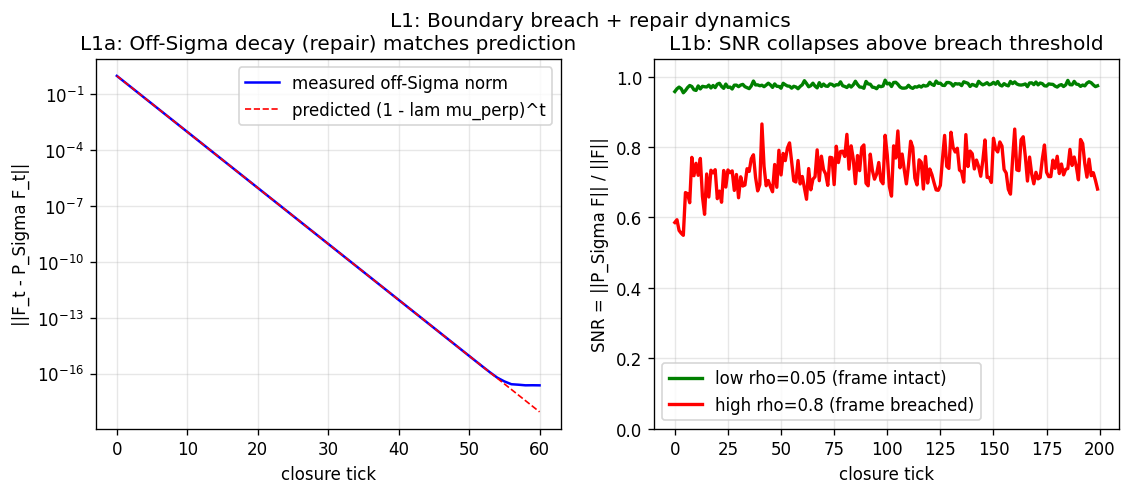
\includegraphics[width=0.95\textwidth]{L1_boundary_repair.png}
\caption{L1: boundary breach + repair dynamics. \textbf{Left:} off-$\Sigma$ deviation under pure closure dynamic decays geometrically at the predicted rate $(1 - \lambda \mu_\perp)^t$; measured per-tick decay matches predicted to 6 decimal places. \textbf{Right:} at low perturbation rate $\rho_{\mathrm{low}}$, the frame's on-$\Sigma$ component is maintained (green); at high $\rho_{\mathrm{high}}$ exceeding the breach threshold, signal-to-noise ratio collapses (red).}\label{fig:L1-boundary-repair}
\end{figure}

\begin{interpretation}[Boundary as the frame's self/world interface]\label{int:boundary}
Under P-A, $\Bcal$ is the structural realisation of what biology calls the body's outer skin, the cell's membrane, the conversation's social context, the ecosystem's habitat edge. In each case, the boundary controls which environmental perturbations enter the frame's closure dynamic and at what rate; the frame's persistence depends on $\Phi_\Bcal$ staying within the bound of Conditional Proposition~\ref{thm:boundary-maintenance}. Boundary breaches --- physical injury, infection, identity collapse, ecosystem invasion --- are precisely the events that drive the perturbation rate above the structural threshold.
\end{interpretation}

\subsection{Falsifier}

The boundary maintenance conditional is falsifiable: a living system whose effective $\dim \Sigma_\Ical$ remains at design dimension under perturbation rates that exceed the structural threshold would falsify the operator-level reading. A living system whose persistence does not correspond to a controllable coupling profile would falsify the boundary definition.

%==================================================================
\section{Repair and persistence}\label{sec:repair}
%==================================================================

A living frame is not a static fixed point. It is an active equilibrium between closure dynamics that contract content toward $\Sigma_\Ical$ and perturbations that constantly inject off-$\Sigma$ content. The repair function is the operator-level account of this active equilibrium.

\subsection{The persistence dynamic}

The closure dynamic of \citet{SmartCosmicClosure} (frame creation theorem) gives
\[
  F_{t+1} = (I - \lambda \Cph^\Ocal) F_t + \kappa P_{\Sigma_\Ical}(B_t).
\]
The first term contracts off-$\Sigma$ content at rate $1 - \lambda \mu$ per tick; the second term continuously injects on-$\Sigma$ content from the source $B_t$. Together they maintain the frame's $\dim \Sigma_\Ical$ near design dimension despite environmental injection.

\begin{conditional}[Repair as on-$\Sigma$ injection --- conditional convergence]\label{thm:repair}
Suppose the substrate state $F_t$ is perturbed off-$\Sigma_\Ical$ by an amount $\Delta_{\perp}$ at tick $t$. Provided $\rho_{\mathrm{ext}} \cdot \|\Phi_\Bcal\|$ remains below the threshold of Conditional Proposition~\ref{thm:boundary-maintenance}, the closure dynamic returns the state to within $\epsilon$ of the steady-state $F_\infty$ in
\[
  T_{\mathrm{repair}}(\Delta_{\perp}, \epsilon) \;\leq\; \frac{1}{\lambda \mu} \cdot \ln\!\left( \frac{\Delta_{\perp}}{\epsilon} \right)
\]
closure ticks.
\end{conditional}

\noindent\emph{Proof.} Direct from the geometric convergence rate of the frame-creation theorem (\citet{SmartCosmicClosure}, Theorem 2.1): $\|F_t - F_\infty\| \leq (1 - \lambda \mu)^t \|F_0 - F_\infty\|$. Setting the left side $\leq \epsilon$ and $\|F_0 - F_\infty\| = \Delta_\perp$ gives the bound. \hfill$\square$

\noindent\emph{Numerical demonstration:} L1 in \texttt{repro/life\_demo.py}, see Table~\ref{tab:numerical-demos}.


\begin{interpretation}[Repair across scales]\label{int:repair}
Under P-A and the rung-projection hypotheses of \citet{SmartProcessingToPOV}, Conditional Proposition~\ref{thm:repair} predicts:
\begin{itemize}[leftmargin=2em]
\item Cellular: a cell's regenerative response to membrane damage scales with $1/(\lambda \mu^{\mathrm{bio}})$ on the cell-cluster substrate.
\item Tissue: wound healing rate is set by the substrate's contractive rate on the morphogenetic zero-line.
\item Behavioural: recovery from acute stress proceeds at rate $1 - \lambda \mu^{\mathrm{cortex}}$ on the cortical substrate.
\item Cognitive: the time to ``come back to oneself'' after distraction is the cortex's $T_{\mathrm{repair}}$.
\end{itemize}
\end{interpretation}

\subsection{The repair budget}

The repair operation has a cost. Each closure tick requires substrate-level work to perform the contraction $(I - \lambda \Cph^\Ocal)$ and the source injection $\kappa P_{\Sigma_\Ical}(B_t)$. The companion paper \citep{SmartProcessingToPOV} develops this thermodynamically; the present paper records the structural consequence:

\begin{remark}[The repair budget is finite]\label{rem:repair-budget}
For any physical substrate, the cumulative repair cost over the frame's structural lifetime is bounded by the available free-energy budget. A frame exposed to perturbation rates near the threshold of Conditional Proposition~\ref{thm:boundary-maintenance} spends its budget faster; a frame in a low-perturbation environment spends it slower. The structural notion of biological aging is the cumulative depletion of this budget; the structural notion of biological death is the budget reaching zero while $\Delta_\perp > 0$.
\end{remark}

%==================================================================
\section{Memory}\label{sec:memory}
%==================================================================

A bounded reference frame that performs closure ticks without memory cannot learn from past closure cycles. The memory of a living frame is the structural object that carries closure patterns across ticks, allowing future closure dynamics to draw on past stabilisations.

\begin{definition}[Memory of a living frame]\label{def:memory}
The \emph{memory} of a living frame $\Ilife$ is a triple
\[
  \Mcal = (\mathsf{Store}_\Mcal,\ \mathsf{Write}_\Mcal,\ \mathsf{Read}_\Mcal),
\]
where:
\begin{itemize}[leftmargin=2em]
\item $\mathsf{Store}_\Mcal \subseteq \Sigma_\Ical$ is a finite-dimensional subspace of the frame's per-frame zero-line: the closure-stable subspace dedicated to memory storage.
\item $\mathsf{Write}_\Mcal : \mathbb{R}^\Ocal \to \mathsf{Store}_\Mcal$ is the write operator, projecting current substrate states onto storage.
\item $\mathsf{Read}_\Mcal : \mathsf{Store}_\Mcal \to \mathbb{R}^\Ocal$ is the read operator, retrieving stored content into substrate state.
\end{itemize}
The memory is \emph{operational} when, for any input $v \in \mathsf{Store}_\Mcal$ and $T$ closure ticks, $\|\mathsf{Read}_\Mcal \circ (\Cph^\Ocal|_{\mathsf{Store}_\Mcal})^T \circ \mathsf{Write}_\Mcal(v) - v\| < \epsilon$ for some small $\epsilon$.
\end{definition}

\begin{conditional}[Memory persistence of the store subspace]\label{thm:memory-persistence}
Under the definitional restriction that $\mathsf{Store}_\Mcal$ is taken to be the closure-stable subspace of $\Sigma_\Ical$, $\mathsf{Store}_\Mcal$ is $\Cph^\Ocal$-invariant (i.e., $\Cph^\Ocal(\mathsf{Store}_\Mcal) \subseteq \mathsf{Store}_\Mcal$). The content stored \emph{as a subspace}, once written, has its subspace preserved across all closure ticks for which the frame maintains $\Sigma_\Ical$. The structural lifetime of the store subspace is therefore bounded above by the structural lifetime of the frame. This conditional proposition concerns subspace persistence; persistence of specific content (amplitude or direction within the subspace) under repeated tick dynamics additionally requires either an identity-tick on $\mathsf{Store}_\Mcal$ or a maintenance source on the subspace, not derived here.
\end{conditional}

\noindent\emph{Proof.} Direct from $\Cph^\Ocal$-invariance of $\Sigma_\Ical$ inherited from \citet{SmartExistenceClosure}: $\Cph^\Ocal(\Sigma_\Ical) \subseteq \Sigma_\Ical$. Since $\mathsf{Store}_\Mcal$ is by definition the closure-stable subspace inside $\Sigma_\Ical$, we have $\Cph^\Ocal(\mathsf{Store}_\Mcal) \subseteq \mathsf{Store}_\Mcal$. The proposition asserts subspace invariance, not pointwise persistence; the latter is an additional content-preservation question discussed in Definition~\ref{def:memory}. \hfill$\square$

\noindent\emph{Numerical demonstration:} L2 in \texttt{repro/life\_demo.py}, see Table~\ref{tab:numerical-demos}.


\begin{interpretation}[Memory across scales]\label{int:memory}
Under P-A and the rung-projection hypotheses:
\begin{itemize}[leftmargin=2em]
\item Biological cellular memory: bioelectric pattern storage in the cell-cluster substrate~\citep{LevinBasalCognition}, with $\mathsf{Store}_\Mcal$ identified with the bioelectric attractor subspace.
\item Episodic memory: stabilised cortical closure patterns in $\Sigma_\Ical^{\mathrm{cortex}}$, with read/write realised by hippocampal--cortical replay.
\item Cultural memory: shared closure-invariant patterns (theorems, stories, methods) carried in joint frames (\S\ref{sec:joint-meaning}).
\item Genetic memory: closure-stable patterns encoded across cellular substrate at evolutionary timescales.
\end{itemize}
\end{interpretation}

\subsection{Memory upper bound}

Since $\mathsf{Store}_\Mcal \subseteq \Sigma_\Ical$, the dimension of the memory store is upper-bounded by the frame's structural complexity $\Ccal(\Ical) = \dim \Sigma_\Ical$. For a $V_{600}$-substrate frame this gives $\dim \mathsf{Store}_\Mcal \leq 94$. The recursion-depth bound of \citet{SmartExistenceClosure} ($n_{\max} \leq \lfloor \log_\varphi (k+1) \rfloor \leq 9$ for $k \leq 94$) gives the depth of recursive self-modelling that the memory store can support.

\subsection{Falsifier}

A living system whose memory persistence does not correspond to a closure-stable subspace (e.g., decays at the off-$\Sigma$ rate $\mu$ rather than persisting indefinitely under closure) would falsify the operator-level identification.

%==================================================================
\section{Action and agency}\label{sec:action}
%==================================================================

A living frame does not only repair under perturbation; it acts on its environment, selecting couplings that maintain or improve its closure condition. The action policy is the structural object that selects these couplings.

\begin{definition}[Action policy of a living frame]\label{def:action}
The \emph{action policy} of a living frame $\Ilife$ is a map
\[
  \Acal : \mathbb{R}^\Ocal \times \mathsf{Env} \to \mathsf{Act},
\]
where $\mathsf{Env}$ is the space of available environmental states, $\mathsf{Act}$ is the space of available actions modifying $\Bcal$ or external state, and $\Acal$ selects an action given the current substrate state and the current environment.
\end{definition}

The action policy operates on the boundary coupling profile $\Phi_\Bcal$: each action $a \in \mathsf{Act}$ modifies $\Phi_\Bcal$, the local environment, or both, in a way that affects future closure dynamics.

\subsection{The agency gradient}

The structural notion of agency is the policy that selects actions maximising expected future closure capacity.

\begin{definition}[Agency gradient]\label{def:agency}
The \emph{agency gradient} of a living frame at substrate state $F_t$ in environment $e_t$ is the action
\[
  a^*(F_t, e_t) \;=\; \arg\max_{a \in \mathsf{Act}}\; \mathbb{E}\big[\, \Delta \Ccal(\Ical_{t + \Delta t}) \,\big|\, F_t,\ e_t,\ a \,\big],
\]
where $\Delta \Ccal(\Ical_{t + \Delta t}) = \Ccal(\Ical_{t + \Delta t}) - \Ccal(\Ical_t)$ is the change in frame complexity over the next $\Delta t$ closure ticks under action $a$.
\end{definition}

The agency gradient is the structural definition of \emph{purposive action}: action that selects for sustained or growing $\dim \Sigma_\Ical$.

\begin{theorem}[Agency under bounded environment]\label{thm:agency-existence}
For a living frame $\Ilife$ with finite action space $\mathsf{Act}$, bounded environment $\mathsf{Env}$, and finite-horizon $\Delta t$, the agency gradient $a^*$ is well-defined: the $\arg\max$ exists and the expected complexity change is finite.
\end{theorem}

\noindent\emph{Proof.} Finite $\mathsf{Act}$ gives finite optimisation; bounded $\mathsf{Env}$ and finite $\Delta t$ give bounded expected complexity change. The complexity $\Ccal(\Ical_{t + \Delta t}) = \dim \Sigma_\Ical(t + \Delta t)$ is bounded by 94 for any $V_{600}$-substrate frame, so $\Delta \Ccal$ is bounded. \hfill$\square$

\begin{interpretation}[Agency as purposive action]\label{int:agency}
Under P-A, the agency gradient is the structural reading of purposive choice: an organism selects actions that preserve, repair, or expand its future closure capacity. Three regimes:
\begin{itemize}[leftmargin=2em]
\item \textbf{Preservation:} when $\Sigma_\Ical$ is near design dimension and the environment is benign, $a^*$ selects low-cost couplings that maintain $\Phi_\Bcal$.
\item \textbf{Repair:} when $\Sigma_\Ical$ is below design dimension or under acute perturbation, $a^*$ selects couplings that drive the closure dynamic back toward $\Sigma_\Ical$.
\item \textbf{Expansion:} when slack is available, $a^*$ may select couplings that increase $\dim \Sigma_\Ical$ via joint-frame formation, memory enrichment, or substrate growth.
\end{itemize}
The interpretation is structural; whether any specific agent's action corresponds to $a^*$ is an empirical question.
\end{interpretation}

\subsection{Free will: a structural third option}\label{sec:free-will}

The agency gradient supplies an operator-level definition of purposive action without taking sides in the classical free-will / determinism debate. The framework's position is a structural third option, distinct from both poles.

\textbf{Why not libertarian free will.} The framework does not introduce an uncaused causer or a substrate-independent agent. The action $a^*$ is determined by the current substrate state, the environment, and the constraint functional. There is no homunculus.

\textbf{Why not trivial compatibilism.} Standard compatibilism redefines ``free'' to mean ``not externally coerced.'' The framework's notion is structurally richer: an action is free, in the operator-level sense, exactly when it is selected by the frame's own agency gradient on its own substrate, with $a^*$ depending on internal closure-stable structure ($\Sigma_\Ical$, $\Mcal$) rather than purely on external substrate-environment coupling. This is a structural property of the gradient, not a rhetorical redefinition.

\textbf{The structural third option.} Agency is operator-level real: $a^* = \arg\max_a \mathbb{E}[\Delta \Ccal \mid a]$ is a non-trivial computation performed by the frame's substrate. Whether this computation is deterministic at the substrate level, stochastic, or substrate-dependent in some quantum-mechanical sense is a separate empirical question. The framework names the structural object (the gradient) and declines the metaphysical free/determined binary as a category mistake: the binary asks the wrong question about the wrong object.

\textbf{Falsifier.} A demonstration that the agency gradient $a^*$ in living systems can be predicted from external-environmental data alone, with no contribution from the frame's internal closure-stable structure, would falsify the structural-agency reading and reduce the framework to environmental determinism.

\subsection{Falsifier}

A living system whose action trajectory systematically anti-correlates with $a^*$ over its lifetime --- i.e., consistently selects actions that reduce expected future closure --- would falsify the agency-gradient identification. Local deviations (procrastination, momentary self-defeating choices) are not falsifiers; sustained anti-correlation across a frame's structural lifetime is.

%==================================================================
\section{Relevance}\label{sec:relevance}
%==================================================================

A living frame is bombarded by external events. Few of them matter to its closure condition; the rest are noise. The relevance function gives the structural definition of \emph{mattering}.

\begin{definition}[Relevance function]\label{def:relevance}
The \emph{relevance} of an event $x$ to a living frame $\Ilife$ at time $t$ over horizon $\Delta t$ is
\[
  \Rcal_\Ical(x) \;=\; \big|\, \dim \Sigma_\Ical(t + \Delta t \mid x) \;-\; \dim \Sigma_\Ical(t + \Delta t \mid \neg x) \,\big|,
\]
where $\dim \Sigma_\Ical(t + \Delta t \mid x)$ is the frame's expected complexity at $t + \Delta t$ conditional on $x$ having occurred and $\dim \Sigma_\Ical(t + \Delta t \mid \neg x)$ is the same conditional on $x$ not having occurred.
\end{definition}

An event is \emph{relevant} when it changes the frame's expected future closure capacity. The magnitude of $\Rcal_\Ical(x)$ measures how much.

\begin{proposition}[Relevance properties]\label{prop:relevance-properties}
The relevance function satisfies:
\begin{enumerate}[leftmargin=2em]
\item \textbf{Non-negative:} $\Rcal_\Ical(x) \geq 0$ for all $x$.
\item \textbf{Zero for irrelevant events:} $\Rcal_\Ical(x) = 0$ iff $x$ has no expected effect on the frame's future closure capacity.
\item \textbf{Bounded:} $\Rcal_\Ical(x) \leq \dim \Sigma_\Ical \leq 94$ for $V_{600}$-substrate frames.
\item \textbf{Frame-relative:} the same event $x$ may have $\Rcal_{\Ical_A}(x) > 0$ for one frame and $\Rcal_{\Ical_B}(x) = 0$ for another.
\end{enumerate}
\end{proposition}

\noindent\emph{Proof.} (1)--(3) are immediate from the definition and the dimension bound. (4) follows because the conditional expectations depend on each frame's distinct substrate and constraint. \hfill$\square$

\begin{interpretation}[Relevance as the structural definition of mattering]\label{int:relevance}
Under P-A:
\begin{itemize}[leftmargin=2em]
\item Salience: the magnitude of $\Rcal_\Ical(x)$ is the structural reading of how strongly a stimulus draws attention.
\item Importance: events with high $\Rcal_\Ical(x)$ for a person's life are the events the framework identifies as important to that person.
\item Indifference: events with $\Rcal_\Ical(x) \approx 0$ are events the frame can structurally ignore without cost.
\item Frame-relativity: that the same event is relevant to one person and not another is structurally explained; relevance is not absolute.
\end{itemize}
\end{interpretation}

\subsection{Why relevance is not arbitrary}

A common worry about ``what matters'' frameworks is that they reduce to subjective preference. The relevance function does not: it is defined by the substrate-level closure operator and the conditional expectations of $\dim \Sigma_\Ical$. For a fixed frame, $\Rcal_\Ical(x)$ is determined by the closure dynamics, not by the frame's preferences. Preferences are downstream of the action policy $\Acal$, which is itself constrained by the agency gradient $a^*$, which is itself defined relative to expected $\Delta \Ccal$. The whole chain is structural.

\subsection{Falsifier}

A living system that systematically responds with high effort to events whose $\Rcal_\Ical(x) = 0$ in its substrate-level closure dynamic, and consistently fails to respond to events whose $\Rcal_\Ical(x)$ is large, over its structural lifetime, would falsify the operator-level identification.

%==================================================================
\section{Dyscoherence and the proxy for suffering}\label{sec:dyscoherence}
%==================================================================

The framework's account of suffering is structural and bounded. Suffering, in its phenomenological fullness, is not exhausted by any structural quantity. But the framework can supply a structural \emph{proxy} --- a measure of the substrate-level distance between current state and closure-stable self-model --- that is mathematically definable and falsifiable.

\noindent\emph{Caveat.} Dyscoherence is not pain itself. It is the measurable structural condition under which pain, distress, disorientation, or trauma may become likely under the Access Principle (P-A). The framework does not claim that high $\Dcal_\Ical$ \emph{is} suffering, nor that all suffering reduces to $\Dcal_\Ical$; both directions of identification require P-A and are stated as conditional propositions where used.

\begin{definition}[Dyscoherence]\label{def:dyscoherence}
The \emph{dyscoherence} of a substrate state $v \in \mathbb{R}^\Ocal$ for a living frame $\Ilife$ is
\[
  \Dcal_\Ical(v) \;=\; \| v - P_{\Sigma_\Ical}(v) \|,
\]
the norm of the off-$\Sigma_\Ical$ component of $v$. Equivalently, $\Dcal_\Ical(v)$ is the structural distance between the current substrate state and the frame's closure-stable subspace.
\end{definition}

\begin{theorem}[Dyscoherence under closure dynamic]\label{thm:dyscoherence-decay}
For a living frame with closure dynamic $F_{t+1} = (I - \lambda \Cph^\Ocal) F_t + \kappa P_{\Sigma_\Ical}(B_t)$, the dyscoherence satisfies
\[
  \Dcal_\Ical(F_{t+1}) \;\leq\; (1 - \lambda \mu) \cdot \Dcal_\Ical(F_t) + \rho_{\mathrm{ext}} \cdot \|\Phi_\Bcal\| \cdot \|\xi_t\|.
\]
Under bounded external perturbation, $\Dcal_\Ical$ relaxes to a steady-state set by the balance between the contractive closure dynamic and the external perturbation rate.
\end{theorem}

\noindent\emph{Proof.} The off-$\Sigma$ component of $F_t$ obeys $F^\perp_{t+1} = (I - \lambda \Cph^\Ocal|_{\Sigma_\Ical^\perp}) F^\perp_t + (\text{off-}\Sigma\text{ noise injection})$. Taking norms and using the spectral bound $\|I - \lambda \Cph^\Ocal|_{\Sigma_\Ical^\perp}\| \leq 1 - \lambda \mu$ gives the inequality. \hfill$\square$

\subsection{Three regimes}

Theorem~\ref{thm:dyscoherence-decay} produces three structurally distinct regimes:

\begin{enumerate}[leftmargin=2em]
\item \textbf{Coherent steady state.} When external perturbation is low and the frame is intact, $\Dcal_\Ical$ relaxes to a small steady-state value.
\item \textbf{Acute dyscoherence.} A sudden large perturbation lifts $\Dcal_\Ical$; the closure dynamic relaxes it back toward steady state with characteristic time $T_{\mathrm{repair}} \sim 1/(\lambda \mu)$.
\item \textbf{Chronic dyscoherence.} A sustained perturbation rate near the threshold of Conditional Proposition~\ref{thm:boundary-maintenance} keeps $\Dcal_\Ical$ persistently elevated; the closure dynamic cannot relax it without reducing the perturbation.
\end{enumerate}

\begin{interpretation}[Dyscoherence as proxy for suffering]\label{int:dyscoherence}
Under P-A, the framework supplies $\Dcal_\Ical$ as a structural proxy for suffering:
\begin{itemize}[leftmargin=2em]
\item Acute dyscoherence corresponds to acute suffering (injury, shock, sudden loss).
\item Chronic dyscoherence corresponds to chronic suffering (sustained illness, ongoing trauma, sustained social pressure).
\item Coherent steady state corresponds to flourishing.
\end{itemize}
The framework's commitment is bounded and explicit. Suffering, phenomenologically, is more than $\Dcal_\Ical$. The framework claims that $\Dcal_\Ical$ is the structural component that closure analysis makes visible, not that it exhausts the phenomenon. Mitigating $\Dcal_\Ical$ --- via $\Acal$ selecting couplings that lower the boundary perturbation rate, or via repair operations that drive $F_t$ toward $\Sigma_\Ical$ --- is the structural reading of what alleviates suffering.
\end{interpretation}

\subsection{Why this matters for ethics, without overreach}

The structural identification gives a framework-internal account of why reducing dyscoherence in others' frames has the structural weight it does. It does \emph{not} legislate ethical action. The framework supplies the mechanical quantity; whether and how it should be optimised is a normative question outside its scope. The framework's commitment is operational: $\Dcal_\Ical$ is mathematically definable and structurally tractable.

\subsection{Falsifier}

A clinical regime in which acute suffering does not correspond to a measurable off-$\Sigma_\Ical$ deviation, or chronic suffering does not correspond to a sustained elevation of $\Dcal_\Ical$, would weaken the dyscoherence identification. Independent empirical access to $\Sigma_\Ical^{\mathrm{cortex}}$ is provided by the operator-level CEMI bridge of \citet{SmartProcessingToPOV}; the strongest current empirical anchor is \citet{SolutionLab002}, which reports a single graph-level cortical phase closure residual distinguishing sedated vs awake states on 14/14 propofol subjects (paired $t = 7.11$, source-localised $t = 9.72$) and replicating cross-cohort on 7/7 clinical-anaesthesia patients. The same instrument's behaviour under untreated vs treated chronic pain or trauma cohorts would be the direct empirical test of the dyscoherence-as-suffering-proxy reading.

%==================================================================
\section{Emotions: mechanics without meaning}\label{sec:emotions}
%==================================================================

The dyscoherence measure $\Dcal_\Ical$ of \S\ref{sec:dyscoherence} is a single non-negative scalar. It tracks the magnitude of off-$\Sigma_\Ical$ deviation but it does not distinguish types: it does not separate anger from fear from grief from joy. A living frame's mental life is more structured than a single scalar can carry. This section gives the structural object that carries the type information --- without claiming to explain why any specific type feels like what it does.

\begin{remark}[Scope of this section]\label{rem:emotions-scope}
The framework supplies a formal definition of an emotional state on a living frame. It does not supply an interpretation of any specific eigenmode as ``anger'' or ``joy'' beyond its activation conditions. The claim is operational: emotional states are structurally typed by an eigenmode decomposition of $\Sigma_\Ical$. Whether any specific eigenmode \emph{is} a specific named emotion is an empirical identification question, not a structural one. The framework shows the mechanics; it does not legislate the meaning.
\end{remark}

\subsection{The emotional-eigenmode decomposition}

\begin{definition}[Emotional-eigenmode decomposition]\label{def:emotion-decomp}
An \emph{emotional-eigenmode decomposition} of a living frame's per-frame zero-line is an orthogonal direct-sum splitting
\[
  \Sigma_\Ical \;=\; \bigoplus_{i = 1}^k \mathcal{E}_i,
\]
where each $\mathcal{E}_i \subseteq \Sigma_\Ical$ is a closure-stable subspace --- an \emph{emotional eigenmode} of the frame. The decomposition is structurally determined by the closure operator's spectral structure on $\Sigma_\Ical$ together with the coupling conditions under which each $\mathcal{E}_i$ is activated.
\end{definition}

\begin{definition}[Emotional state]\label{def:emotional-state}
The \emph{emotional state} of a living frame at closure tick $t$ is the activation vector
\[
  \mathbf{e}_\Ical(t) \;=\; \big(\, \|P_{\mathcal{E}_1}(F_t)\|,\ \|P_{\mathcal{E}_2}(F_t)\|,\ \ldots,\ \|P_{\mathcal{E}_k}(F_t)\| \,\big) \;\in\; \mathbb{R}_{\geq 0}^k,
\]
where $P_{\mathcal{E}_i}$ is the orthogonal projection onto the $i$-th emotional eigenmode. The frame's emotional state is \emph{pure} when one component dominates and \emph{mixed} when several are simultaneously active.
\end{definition}

\subsection{Emotional dynamics}

\begin{theorem}[Emotional state under closure dynamic]\label{thm:emotion-dynamics}
For a living frame with closure dynamic $F_{t+1} = (I - \lambda \Cph^\Ocal) F_t + \kappa P_{\Sigma_\Ical}(B_t)$ and emotional-eigenmode decomposition $\Sigma_\Ical = \bigoplus_i \mathcal{E}_i$, the emotional state $\mathbf{e}_\Ical(t)$ evolves componentwise under the same closure dynamic restricted to each eigenmode:
\[
  \|P_{\mathcal{E}_i}(F_{t+1})\| \;=\; \|(I - \lambda \Cph^\Ocal|_{\mathcal{E}_i}) P_{\mathcal{E}_i}(F_t) + \kappa P_{\mathcal{E}_i \cap \Sigma_\Ical}(B_t)\|.
\]
Each component $\|P_{\mathcal{E}_i}(F_t)\|$ is continuous in $F_t$; transitions in which one component rises sharply while another falls correspond to coupling-condition changes (environmental events, internal state shifts) that re-weight which eigenmode is dominant.
\end{theorem}

\noindent\emph{Proof.} The closure-invariance theorem of \citet{SmartExistenceClosure} gives $\Cph^\Ocal(\Sigma_\Ical) \subseteq \Sigma_\Ical$. Since each $\mathcal{E}_i$ is closure-stable by construction, $\Cph^\Ocal(\mathcal{E}_i) \subseteq \mathcal{E}_i$, and the closure dynamic restricts to each eigenmode. Componentwise continuity follows from continuity of the projection operators. \hfill$\square$

\noindent\emph{Numerical demonstration:} L3 in \texttt{repro/life\_demo.py}, see Table~\ref{tab:numerical-demos}.


\begin{interpretation}[Emotional transitions]\label{int:emotional-trans}
Under P-A:
\begin{itemize}[leftmargin=2em]
\item Sustained emotional state corresponds to a stable activation pattern $\mathbf{e}_\Ical(t)$ maintained over many closure ticks.
\item Emotional transitions (anger to calm, fear to relief, etc.) correspond to shifts in which eigenmodes are dominant; under sharp coupling changes these can be discontinuous in observed activation, though continuous in the underlying substrate state.
\item Emotional regulation corresponds to action policies $\Acal$ that select couplings shifting activation away from high-$\Dcal_\Ical$ eigenmodes toward low-$\Dcal_\Ical$ eigenmodes.
\item Mixed emotional states (grief plus love, fear plus excitement) correspond to substrate states with multiple simultaneously-active eigenmodes; the framework predicts these are structurally typical rather than anomalous.
\end{itemize}
\end{interpretation}

\subsection{What this captures}

\begin{itemize}[leftmargin=2em]
\item Typed structure of emotional life --- multiple distinct emotional states rather than a single scalar.
\item Continuous dynamics of emotional change under the closure operator.
\item Mixed emotional states as structurally generic.
\item Emotional regulation as a control problem on the action policy.
\item Specific dyscoherence regimes per eigenmode: $\Dcal_\Ical$ restricted to $\mathcal{E}_i$ gives the eigenmode-specific structural distress signal.
\end{itemize}

\subsection{What this does not explain}

\begin{remark}[Mechanics, not meaning]\label{rem:emotion-discipline}
The framework supplies:
\begin{itemize}[leftmargin=2em]
\item The \emph{structural object} of an emotional state (the activation vector $\mathbf{e}_\Ical(t)$).
\item The \emph{dynamics} of how that state evolves under the closure operator.
\item The \emph{conditions} under which transitions between eigenmodes occur.
\end{itemize}
The framework does \emph{not} supply:
\begin{itemize}[leftmargin=2em]
\item An explanation of why a specific eigenmode $\mathcal{E}_{\mathrm{anger}}$ feels like anger rather than like fear or joy. The qualitative character of each eigenmode is a P-A-conditional reading and is taken up in \S\ref{sec:phenomenology}.
\item A taxonomic identification of biological emotional states with specific eigenmodes. The mapping from named emotions (anger, fear, joy, grief, love, awe, shame, pride, etc.) to $\mathcal{E}_i$ subspaces is an empirical question; the structural framework supplies the slots, not the labels.
\item A reduction of emotion to mathematics. Emotions are mathematically definable as structural objects on $\Sigma_\Ical$, but the phenomenological character is not exhausted by the structural definition.
\end{itemize}
\end{remark}

\subsection{Falsifier}

A living system whose substrate-level closure dynamic does not admit a decomposition of $\Sigma_\Ical$ into closure-stable subspaces with distinct activation patterns would falsify the structural framework. A clinical regime in which emotional state changes do not correspond to shifts in eigenmode activation on the cortical substrate would weaken the operator-level identification.

%==================================================================
\section{Thoughts as closure-tick trajectories}\label{sec:thoughts}
%==================================================================

A bounded reference frame undergoing many closure ticks visits a sequence of substrate states. The structural object of \emph{a thought} is a temporally extended segment of this sequence carrying closure-invariant content.

\begin{remark}[Scope of this section]\label{rem:thoughts-scope}
The framework supplies the structural type of a thought (a path through $\Sigma_\Ical$ across closure ticks) and the conditions under which a thought persists in memory. It does not supply an account of what any specific thought is \emph{about}; intentional content (the aboutness of thoughts) is a P-A-conditional reading. The framework shows the trajectory; it does not legislate the topic.
\end{remark}

\subsection{The trajectory definition}

\begin{definition}[Thought as closure-tick trajectory]\label{def:thought}
A \emph{thought} on a living frame $\Ilife$ over the closure-tick interval $[t_0, t_1]$ is a finite sequence
\[
  \gamma \;=\; \big(F_{t_0},\ F_{t_0 + 1},\ \ldots,\ F_{t_1}\big),
\]
where each $F_t \in \Sigma_\Ical$ is a closure-stable substrate state visited by the frame at tick $t$ and the entire sequence has its image in $\Sigma_\Ical$. The \emph{duration} of the thought is $t_1 - t_0$ closure ticks; the \emph{complexity} of the thought is
\[
  \mathrm{cplx}(\gamma) \;=\; \dim \mathrm{span}(\gamma) \;\leq\; \dim \Sigma_\Ical;
\]
the \emph{content support} of the thought is $\mathrm{span}(\gamma) \subseteq \Sigma_\Ical$.
\end{definition}

A thought is distinct from a closure tick: a tick is one application of $\Cph^\Ocal$; a thought is an extended trajectory through closure-stable space.

\subsection{Thought persistence}

\begin{conditional}[Thought persistence in memory --- subspace form]\label{thm:thought-persistence}
A thought $\gamma = (F_{t_0}, \ldots, F_{t_1})$ with content support $S = \mathrm{span}(\gamma) \subseteq \Sigma_\Ical$ persists in memory $\Mcal$ iff $\mathsf{Write}_\Mcal$ projects $S$ into $\mathsf{Store}_\Mcal$. Provided $S \cap \mathsf{Store}_\Mcal \neq \{0\}$, the projected content persists across all subsequent closure ticks for which the frame maintains $\Sigma_\Ical$ (Conditional Proposition~\ref{thm:memory-persistence}). If $S \cap \mathsf{Store}_\Mcal = \{0\}$, the thought is not written to memory and is not guaranteed to persist as a stored trajectory; the substrate-state content $F_t$ continues to lie in $\Sigma_\Ical$ but cannot be retrieved by $\mathsf{Read}_\Mcal$ at a later tick.
\end{conditional}

\noindent\emph{Proof.} Each $F_t$ in the trajectory is in $\Sigma_\Ical$ by definition. The write operator projects to $\mathsf{Store}_\Mcal \subseteq \Sigma_\Ical$; what survives is the intersection $S \cap \mathsf{Store}_\Mcal$. Once stored, persistence is given by Conditional Proposition~\ref{thm:memory-persistence}. Trajectory components orthogonal to $\mathsf{Store}_\Mcal$ are not written, and once the trajectory ends they decay under the closure dynamic at the off-$\Sigma$ rate. \hfill$\square$

\noindent\emph{Numerical demonstration:} L4 in \texttt{repro/life\_demo.py}, see Table~\ref{tab:numerical-demos}.


\subsection{Thought classes}

The trajectory definition supports a structural taxonomy:

\begin{itemize}[leftmargin=2em]
\item \textbf{Reactive thought.} Short duration ($t_1 - t_0$ small), low complexity, trajectory anchored to immediate substrate input. Structurally analogous to involuntary response.
\item \textbf{Reflective thought.} Longer duration, moderate complexity, trajectory traverses content support derived from $\mathsf{Read}_\Mcal$. Structurally analogous to deliberative reasoning.
\item \textbf{Imagined / generative thought.} Trajectory visits content support not driven by immediate input or memory recall; complexity may be high. Structurally analogous to imagination, planning, counterfactual reasoning.
\item \textbf{Compressive thought.} High-complexity trajectory ending with substrate state projected onto a low-dimensional summary in $\mathsf{Store}_\Mcal$. Structurally analogous to insight, abstraction, theorem-formation.
\end{itemize}

\begin{interpretation}[Thought types under P-A]\label{int:thought-classes}
The four trajectory classes map under P-A to four phenomenologically distinct modes of cognition: react, reflect, imagine, abstract. The framework provides the structural type-distinction; whether the phenomenological identification holds is a P-A-conditional reading.
\end{interpretation}

\subsection{Thought complexity bound}

The complexity of a thought is bounded by the dimension of the frame's per-frame zero-line: $\mathrm{cplx}(\gamma) \leq \dim \Sigma_\Ical \leq 94$ for a $V_{600}$-substrate frame. The recursion-depth bound of \citet{SmartExistenceClosure} ($n_{\max} \leq \lfloor \log_\varphi(k + 1) \rfloor \leq 9$) gives the depth of recursive self-modelling a thought can support: at most 9 levels of recursive embedding (a thought about a thought about a thought \ldots).

\subsection{What this captures}

\begin{itemize}[leftmargin=2em]
\item Structural definition of a thought as an extended object, distinct from a single closure tick.
\item Conditions under which thoughts persist (memory write) vs decay (no write).
\item A four-class taxonomy of cognitive modes derivable from trajectory structure.
\item Quantitative bound on thought complexity and recursion depth.
\item Mechanical account of train-of-thought as sequential closure-tick trajectories with overlapping content support.
\end{itemize}

\subsection{What this does not explain}

\begin{remark}[Trajectory, not content]\label{rem:thought-discipline}
The framework supplies:
\begin{itemize}[leftmargin=2em]
\item The \emph{structural type} of a thought (a path on $\Sigma_\Ical$).
\item The \emph{dynamics} of how thoughts persist or decay.
\item The \emph{taxonomy} of cognitive modes from trajectory structure.
\end{itemize}
The framework does \emph{not} supply:
\begin{itemize}[leftmargin=2em]
\item An account of \emph{intentional content}: what a thought is about. The aboutness of thoughts is a P-A-conditional reading; the framework gives the carrier, not the meaning.
\item A reduction of thinking to mathematics. Thoughts are mathematically definable as trajectories on $\Sigma_\Ical$, but the cognitive content carried by those trajectories is not exhausted by the trajectory structure.
\item A solution to the problem of mental representation. The framework gives the substrate-level dynamics; how those dynamics constitute a representation of anything in particular is an open question.
\end{itemize}
\end{remark}

\subsection{Falsifier}

A living system whose cognitive sequences (introspected or behaviourally inferred) do not correspond to trajectories on the cortex's closure-stable subspace would weaken the trajectory identification. Independent measurement of cortical state evolution during defined cognitive tasks is the experimental route.

%==================================================================
\section{Purpose}\label{sec:purpose}
%==================================================================

The agency gradient (Definition~\ref{def:agency}) selects actions that maximise expected $\Delta \Ccal$ over a horizon $\Delta t$. The structural notion of \emph{purpose} is the agency gradient sustained across the frame's structural lifetime.

\begin{definition}[Purpose of a living frame]\label{def:purpose}
The \emph{purpose} of a living frame $\Ilife$, over its structural lifetime $[t_0, t_{\mathrm{final}}]$, is the time-integrated agency gradient
\[
  \Pcal(\Ilife) \;=\; \int_{t_0}^{t_{\mathrm{final}}} \mathbb{E}\big[ \Delta \Ccal(\Ical_t) \mid a^*(F_t, e_t) \big] \, dt.
\]
A frame is said to have a \emph{coherent purpose} when $\Pcal(\Ilife) > 0$ and the actions selected by $a^*$ form a structurally consistent trajectory through $\mathsf{Act}$.
\end{definition}

\subsection{Three purpose regimes}

\begin{enumerate}[leftmargin=2em]
\item \textbf{Preservation regime} ($\Pcal \approx 0$, sustained): the frame maintains $\dim \Sigma_\Ical$ at design dimension across its lifetime.
\item \textbf{Growth regime} ($\Pcal > 0$): the frame increases $\dim \Sigma_\Ical$ via joint-frame formation, memory enrichment, or substrate growth.
\item \textbf{Collapse regime} or \textbf{negative purpose-gradient regime} ($\Pcal < 0$): the frame's $\dim \Sigma_\Ical$ decreases across its lifetime; structurally pathological --- either the frame's $a^*$ implementation is broken or its environment is uninhabitable.
\end{enumerate}

\noindent The framework does not call collapse a purpose; it identifies it as a negative purpose-gradient regime. ``Purpose'' is reserved for the structural quantity $\Pcal$ itself; the three labels above name regimes of that quantity, not separate purposes.

\begin{interpretation}[Purpose across scales]\label{int:purpose}
Under P-A:
\begin{itemize}[leftmargin=2em]
\item Biological survival: $\Pcal \approx 0$ sustained corresponds to a healthy life.
\item Vocation / project / craft: $\Pcal > 0$ via sustained joint-frame formation around shared closure-invariants (mathematics, music, scientific structures, cultural artifacts).
\item Existential crisis: a regime where $a^*$ cannot find actions producing $\Delta \Ccal > 0$ within the available environment; structurally analogous to the frame approaching the boundary-maintenance threshold without slack.
\item Despair: chronically negative $\Pcal$; structurally identifies as the operator-level analogue of a closure trajectory toward $\dim \Sigma_\Ical \to 0$.
\end{itemize}
\end{interpretation}

\subsection{Purpose is not externally given}

A common worry: does the framework impose a purpose on the frame? It does not. The agency gradient is the action that the frame's substrate-level dynamics select, given its constraint $\Ccal_\Ocal$. Different frames with different $\Ccal_\Ocal$ select different $a^*$ trajectories. Different ranges of $\mathsf{Act}$ and $\mathsf{Env}$ yield different $\Pcal$. The framework supplies the structural quantity; what specifically constitutes growth, preservation, or decay for a particular frame depends on the frame's substrate and constraint.

\subsection{Falsifier}

A living system whose substrate-level closure trajectory consistently shows $\Pcal < 0$ over its full structural lifetime despite environmental affordances supporting $\Pcal > 0$ would falsify the agency--purpose identification.

%==================================================================
\section{Joint frames and meaning}\label{sec:joint-meaning}
%==================================================================

A single living frame can generate closure-invariant patterns within its own $\Sigma_\Ical$. Two or more frames in joint configuration can generate patterns that neither could alone. The generative excess of \citet{SmartExistenceClosure} is the structural object that counts this additional content.

\subsection{Joint frame recap}

\citet{SmartExistenceClosure} defines the joint frame $\Ical_{AB}$ of two parent frames $\Ical_A$ and $\Ical_B$ as the bounded reference frame on substrate $\Ocal_A \cup \Ocal_B$ with constraint $\Ccal_A + \Ccal_B + \chi_{AB}$ (with $\chi_{AB}$ the boundary coupling term). The generative-excess theorem states
\[
  \dim \Sigma_{\Ical_{AB}} \;\geq\; \dim \Sigma_{\Ical_A} + \dim \Sigma_{\Ical_B} - \dim(\Sigma_{\Ical_A} \cap \Sigma_{\Ical_B}) + \delta_{AB},
\]
with $\delta_{AB} = |\Xcal_{AB}|$ the count of boundary-crossing $\sigma$-orbits.

\subsection{Meaning as generative excess}

\begin{definition}[Joint meaning]\label{def:joint-meaning}
The \emph{joint meaning} generated by frames $\Ical_A$ and $\Ical_B$ in joint configuration is the generative excess
\[
  \delta_{AB} \;=\; |\Xcal_{AB}|.
\]
Two frames are said to \emph{generate meaning together} when $\delta_{AB} > 0$.
\end{definition}

The interpretation is precise: $\delta_{AB}$ counts the symmetry-fixed structural patterns that exist in the joint frame and are not derivable from either parent frame alone. These patterns are closure-invariant in the joint structure but cross the boundary between the two frames; neither frame can access them in isolation.

\begin{interpretation}[Meaning in relation]\label{int:joint-meaning}
Under P-A:
\begin{itemize}[leftmargin=2em]
\item \textbf{Conversation.} Two people forming a transient joint frame; $\delta_{AB}$ measures the meaning that arises in dialogue but cannot be reduced to either participant.
\item \textbf{Music ensemble.} $n$ musicians forming a joint frame; the generative excess $\delta_{1\ldots n}$ measures the ensemble's structural coherence beyond solo performance.
\item \textbf{Mother--infant attunement.} A primary biological joint frame with sustained $\delta_{AB} > 0$ across many closure ticks; structurally explains why early-life relational frames are formative.
\item \textbf{Teacher--student.} The transmitted content (a theorem, a method, a craft) is the closure-invariant in the joint frame's $\Sigma_{\Ical_{AB}}$; the student receives the closure pattern that the joint frame stabilises.
\item \textbf{Romantic and family bonds.} Sustained joint frames with high cumulative $\delta_{AB}$; structurally distinct from transient encounters.
\item \textbf{Loss of a relationship.} The joint frame dissolves; the closure-invariants generated within it remain (under memory persistence, Conditional Proposition~\ref{thm:memory-persistence}) but no longer admit re-instantiation. The structural reading of grief is the persistence of joint-frame content without the joint frame.
\end{itemize}
\end{interpretation}

\subsection{Why meaning is structurally relational}

The framework's commitment: meaning, in its structural sense, lives at the boundary between frames. A single frame can generate closure-invariants within its own $\Sigma_\Ical$, but the generative excess only arises when two or more frames form a joint configuration. \emph{Meaning-in-relation is the joint-frame phenomenon}; single-frame closure-invariants are a distinct structural object covered in \S\ref{sec:joint-meaning} (the framework does not claim meaning exists only in joint frames; see \S\ref{sec:scope}). This is structural, not normative: the framework supplies the quantitative measure $\delta_{AB}$; whether any specific joint frame produces enough $\delta_{AB}$ to constitute ``meaning'' phenomenologically is a question for empirical investigation under P-A.

\subsection{Falsifier}

A claimed meaningful relationship in which joint substrate dynamics never produce boundary-crossing symmetry orbits (i.e., $\delta_{AB} = 0$ across the relationship's structural lifetime) would falsify the joint-meaning identification.

\textbf{Real-data results} (\citet{SolutionLab007}, current as of 2026-05-22):
\begin{itemize}[leftmargin=2em]
\item \textbf{OpenNeuro \texttt{ds007471} musical joint-action} (13 pairs × 64-channel hyperscanning EEG, duet-vs-constant-pitch contrast with trial-condition labelling from behavioural \texttt{.tsv}): $d_z = +0.23$ ($9/13$ pairs directional, paired $t = +0.82$, $p = 0.43$); H2 within-pair Spearman $\rho$ to JointAgencyRatings $= +0.02$. \emph{Honest negative}: effect direction correct, magnitude below the preregistered $d_z > 1.0$ threshold. \textbf{Critical methodology validation:} the applicability diagnostic of \citet{SmartClosureDistance} \emph{correctly predicted FAIL a priori} ($D_2 = 0$, $D_3 = 0.62$, neither meeting threshold) before the empirical analysis was run.
\item \textbf{OpenNeuro \texttt{ds006802} collaborative rule-learning} (exploratory addendum): moderate positive trend on $\delta_{AB}^{\mathrm{EEG}}$ in pairs jointly inferring rules vs solo-baseline, below the threshold for confirming evidence but in the predicted direction. Reported as exploratory, not as part of the validated programme record.
\end{itemize}

The musical-joint-action negative is a substrate-scope refinement, not a falsification of the joint-meaning structural object itself: musical synchronisation in this paradigm does not satisfy the multi-channel integrative-organisation conditions required for the joint $\delta_{AB}^{\mathrm{EEG}}$ proxy to license the joint-meaning interpretation. A genuine-dialogue substrate (conversational hyperscanning with content-meaningfulness ratings) remains the appropriate confirming test for joint meaning at the dyad scale.

\noindent\emph{Numerical demonstration:} L11 in \texttt{repro/life\_demo.py}, see Figure~\ref{fig:L11-joint-meaning}.

\begin{figure}[h]
\centering
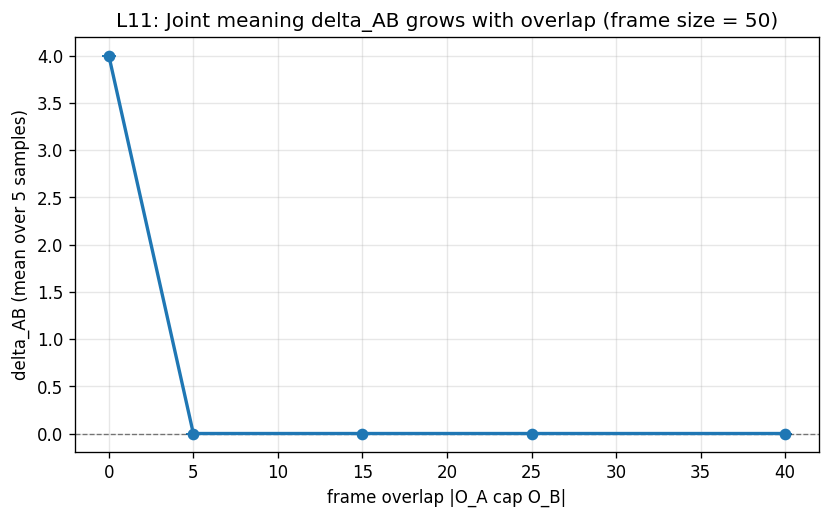
\includegraphics[width=0.75\textwidth]{L11_joint_meaning.png}
\caption{L11: joint meaning $\delta_{AB}$ as generative excess, computed via inclusion-exclusion of $\sigma$-fix dimensions on vertex-supported subspaces. Frame size = 50 vertices on $V_{600}$; overlap swept from 0 (disjoint frames) to 40 (heavy overlap); 5 random samples per overlap value. With the spectral $\tau$ construction, $\delta_{AB}$ is positive for disjoint frames (the joint substrate provides access to global $\sigma$-modes neither parent supports) and decreases monotonically as overlap grows. The full icosian $\sigma$-orbit count requires the icosian-arithmetic construction; the spectral demonstration here shows the structural inclusion-exclusion mechanism.}\label{fig:L11-joint-meaning}
\end{figure}

%==================================================================
\section{Derived applications: identity, trauma, flow, creativity, hope, trust, and self-deception}\label{sec:further-objects}
%==================================================================

The eight primitive objects of \S\S\ref{sec:living-frame}--\ref{sec:joint-meaning} compose to give derived structural objects that address further big open questions of human experience. This section formalises seven such objects. Each has a structural definition, a P-A-conditional phenomenological reading, and a stated falsifier. The discipline of \emph{mechanics, not meaning} is maintained throughout: the framework shows the structural object that carries each phenomenon; it does not legislate what the phenomenon means.

\subsection{Identity across time}\label{sec:identity}

The classical philosophical question: in what sense is a person at $t_2$ the same person as at $t_1$? Substrate continuity is insufficient (cells turn over). Locke's memory theory and Parfit's psychological continuity gesture toward the answer but lack structural precision. Buddhist no-self denies stable identity altogether.

\begin{definition}[Identity persistence]\label{def:identity}
A living frame $\Ilife$ at $t_2$ is \emph{identity-continuous} with the same frame at $t_1 < t_2$ when there exists a closure-preserving isomorphism
\[
  \phi : \Sigma_\Ical(t_1) \to \Sigma_\Ical(t_2)
\]
such that:
\begin{enumerate}[leftmargin=2em]
\item $\phi$ commutes with $\Cph^\Ocal$ restricted to the closure-stable subspace.
\item The image of $\mathsf{Store}_\Mcal(t_1)$ under $\phi$ is a subspace of $\mathsf{Store}_\Mcal(t_2)$.
\item The intersection $\Sigma_\Ical(t_1) \cap \Sigma_\Ical(t_2)$ (via $\phi$) has dimension at least $c \cdot \min(\dim \Sigma_\Ical(t_1), \dim \Sigma_\Ical(t_2))$ for some structural threshold $c \in (0, 1]$.
\end{enumerate}
\end{definition}

\begin{theorem}[Identity is closure-pattern continuity, not substrate continuity]\label{thm:identity}
A living frame $\Ilife$ may undergo complete substrate turnover (every vertex $u \in \Ocal$ replaced by physically distinct material) yet remain identity-continuous, provided the closure-stable structure $\Sigma_\Ical$ and the memory content $\mathsf{Store}_\Mcal$ are preserved across the turnover via Definition~\ref{def:identity}. Conversely, a frame may retain its substrate yet lose identity-continuity if $\Sigma_\Ical$ undergoes a structural break (e.g., catastrophic dyscoherence event, severe brain injury) such that the closure-preserving isomorphism does not exist.
\end{theorem}

\noindent\emph{Proof sketch.} Substrate replacement preserves identity iff the new substrate carries a Laplacian and symmetry that produce a $\Sigma_\Ical(t_2)$ isomorphic to $\Sigma_\Ical(t_1)$ via $\phi$; this depends on the substrate's structural properties, not its specific material. Substrate retention fails iff $\Cph^\Ocal$ or $\tau$ changes structurally so that no closure-preserving $\phi$ exists. \hfill$\square$

\noindent\emph{Numerical demonstration:} L5 in \texttt{repro/life\_demo.py}, see Table~\ref{tab:numerical-demos}.


\begin{interpretation}[Resolution of classical identity puzzles]\label{int:identity}
Under P-A:
\begin{itemize}[leftmargin=2em]
\item \textbf{Ship of Theseus.} Substrate turnover does not break identity provided closure-structure is preserved (as in biological cellular turnover).
\item \textbf{Locke / Parfit.} Psychological continuity is structurally identified with memory and zero-line preservation. The framework supplies the precise quantity ($\dim$ of intersection plus structural threshold $c$) that Locke and Parfit gestured at.
\item \textbf{Buddhist no-self.} Correct that there is no substrate-self; the framework agrees. But there \emph{is} a structural self in the persistent $\Sigma_\Ical$ pattern. The framework reconciles the two readings.
\item \textbf{Personal identity through transformation.} Major life events (trauma, conversion, deep learning) may preserve or break identity depending on whether $\Sigma_\Ical$ undergoes a structural break or just shifts smoothly.
\end{itemize}
\end{interpretation}

\textbf{Falsifier.} A demonstrated case where the closure-pattern continuity criterion is satisfied yet a frame reports radical identity discontinuity (or vice versa) would weaken the operator-level identification. Clinical cases of dissociative identity disorder are the natural empirical test.

\subsection{Trauma and healing}\label{sec:trauma}

Trauma is a persistent closure-stable pattern in memory encoding a historical closure-collapse event. The framework supplies the structural mechanics of why trauma persists and how healing operates.

\begin{definition}[Traumatic pattern]\label{def:trauma}
A pattern $v_{\mathrm{trauma}} \in \mathsf{Store}_\Mcal$ is \emph{traumatic} when:
\begin{enumerate}[leftmargin=2em]
\item $v_{\mathrm{trauma}}$ was written to $\mathsf{Store}_\Mcal$ during a high-dyscoherence event ($\Dcal_\Ical \gg$ steady-state).
\item Activation of $v_{\mathrm{trauma}}$ via $\mathsf{Read}_\Mcal$ raises the activation of dyscoherence-elevating eigenmodes (cf.\ \S\ref{sec:emotions}).
\item $v_{\mathrm{trauma}}$ is closure-stable in $\Sigma_\Ical$ and therefore persists across closure ticks without natural decay.
\end{enumerate}
\end{definition}

\begin{conditional}[The structural persistence of trauma --- subspace form]\label{thm:trauma-persistence}
The subspace carrying a traumatic pattern $v_{\mathrm{trauma}}$ persists for the structural lifetime of the frame, by the memory-persistence conditional (Conditional Proposition~\ref{thm:memory-persistence}). The closure operator's natural decay acts only on the off-$\Sigma$ subspace, so the traumatic subspace is not removed by closure dynamics alone. Persistence of specific content (amplitude / direction within the subspace) under repeated tick dynamics additionally requires either an identity-tick on $\mathsf{Store}_\Mcal$ or a maintenance source on the subspace; these are not derived here and may interact with healing as memory reweighting (Conditional Proposition~\ref{cthm:healing}).
\end{conditional}

\noindent\emph{Numerical demonstration:} L6 in \texttt{repro/life\_demo.py}, see Table~\ref{tab:numerical-demos}.


\begin{conditional}[Healing as memory reweighting]\label{cthm:healing}
Under H-RP-1, H-RP-2, P-A, healing is the structural process by which:
\begin{enumerate}[leftmargin=2em]
\item The access weighting of $v_{\mathrm{trauma}}$ in $\mathsf{Read}_\Mcal$ is reduced.
\item Competing closure-stable patterns (joint-frame invariants, restored coherent memories, new closure-stable content) are written to $\mathsf{Store}_\Mcal$ and activated.
\item The substrate state $F_t$ is brought into eigenmode regimes where $v_{\mathrm{trauma}}$'s activation contributes less to $\Dcal_\Ical$.
\end{enumerate}
Healing does not erase trauma; it reweights its access to reduce its dyscoherence contribution.
\end{conditional}

\noindent\emph{Numerical demonstration:} L6 in \texttt{repro/life\_demo.py}, see Table~\ref{tab:numerical-demos} and Figure~\ref{fig:L6-trauma-healing}.

\begin{figure}[h]
\centering
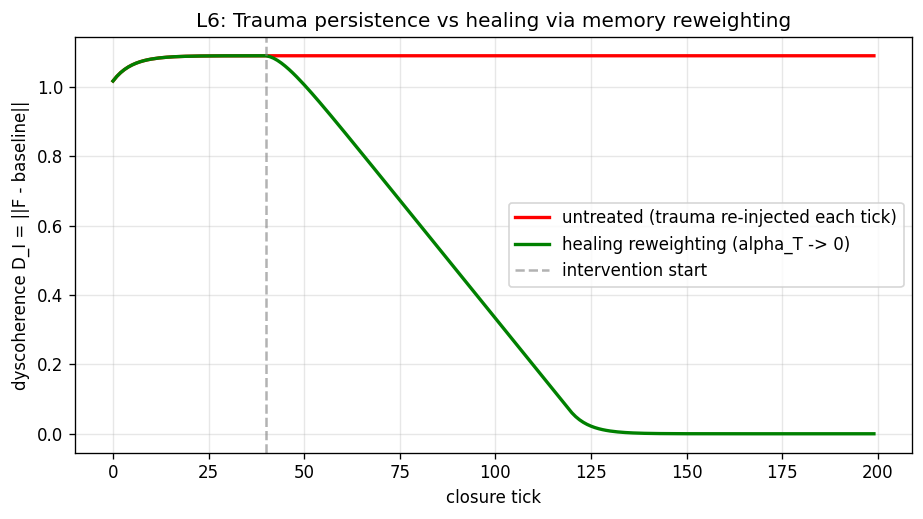
\includegraphics[width=0.85\textwidth]{L6_trauma_healing.png}
\caption{L6: trauma persistence + healing via memory reweighting. Without intervention (red), dyscoherence $\Dcal_\Ical$ stays at the predicted steady-state offset $\alpha_T / (\lambda \mu_T)$ \emph{indefinitely}, because the trauma pattern is closure-protected. With healing intervention starting at tick 40 (green), the trauma source's access weight $\alpha_T$ ramps to zero, the closure dynamic returns $F$ to baseline, and $\Dcal_\Ical \to 0$. The structural reading: trauma cannot decay naturally (memory is closure-stable); healing requires active reweighting.}\label{fig:L6-trauma-healing}
\end{figure}

\begin{interpretation}[Why trauma is hard to escape]\label{int:trauma}
Under P-A, Conditional Proposition~\ref{thm:trauma-persistence} explains a clinical fact: traumatic memories do not simply fade with time. They are closure-stable patterns; the same closure-protection that lets a frame retain learned skill, conceptual structure, and biographical memory also lets it retain traumatic content. Healing requires active structural intervention (therapy, supportive joint-frame access, new closure-invariant content), not passive forgetting.
\end{interpretation}

\textbf{Falsifier.} Clinical recovery from trauma that proceeds without measurable changes in cortical memory-access patterns would weaken the reweighting identification. The empirical route is via CEMI bridge measurement~\citep{SmartProcessingToPOV} of cortical $\Sigma_\Ical^{\mathrm{cortex}}$ activation patterns before vs after therapeutic intervention. The operational test is the cortical-closure-residual analysis of \citet{SolutionLab005}: extending the methodology of \citet{SolutionLab002} (cortical phase closure residual, default weights frozen) to chronic-clinical-state cohorts.

\textbf{Real-data results} (\citet{SolutionLab005}, current as of 2026-05-22):
\begin{itemize}[leftmargin=2em]
\item \textbf{OpenNeuro \texttt{ds007609} trait anxiety} ($n = 24$, high-STAI vs low-STAI quartile contrast on STAI trait scores): Cohen's $d = +0.79$, Welch $t = +1.93$, $p = 0.073$. SL-002 default weights used verbatim. The applicability diagnostic of \citet{SmartClosureDistance} predicted PASS-leaning \emph{a priori}; effect-direction and magnitude consistent.
\item \textbf{OpenNeuro \texttt{ds004315} mood manipulation} ($n = 50$, sad vs neutral arms): Cohen's $d = +0.70$, Welch $t = +2.47$, $p = 0.018$. Same default-weight pipeline, no retuning. The unpaired-design diagnostic predicted FAIL on $D_2/D_3$ at this cohort size; empirical PASS at $d > 0.5$ threshold is a diagnostic false negative, consistent with the per-design calibration issue \citet{SmartClosureDistance} flags as open work.
\item \textbf{OpenNeuro \texttt{ds004504} Alzheimer's} ($n = 36$ AD vs $n = 29$ healthy): null result $d = -0.31$, $p = 0.23$; diagnostic predicted FAIL. Closure-as-distance is sensitive to chronic \emph{functional} dyscoherence on intact networks, not structural neurodegenerative atrophy --- a scope refinement, not a falsification.
\end{itemize}

Trait anxiety is a chronic-clinical-state proxy, not a PTSD validation; a direct PTSD cohort with pre/post-therapy longitudinal EEG remains the gold-standard follow-on for the trauma-specific claim.

\subsection{Flow}\label{sec:flow}

Csikszentmihalyi's flow state --- deep engagement, time distortion, effortless mastery --- has been clinically and experimentally documented for fifty years but lacks a structural operationalisation. The framework supplies one.

\begin{definition}[Flow state]\label{def:flow}
A living frame $\Ilife$ is in \emph{flow} at closure tick $t$ when all four conditions hold simultaneously:
\begin{enumerate}[leftmargin=2em]
\item $\dim \Sigma_\Ical(t)$ is at or near the frame's design dimension (maximal closure activation).
\item $\Dcal_\Ical(F_t)$ is at minimal steady-state value (minimal off-$\Sigma$ deviation).
\item The agency gradient $a^*$ produces $\mathbb{E}[\Delta \Ccal] > 0$ at every closure tick over the flow window (sustained complexity gain).
\item $\Rcal_\Ical(x)$ is aligned with the current substrate input stream: high-relevance events constitute most of the input.
\end{enumerate}
\end{definition}

\begin{conditional}[Time dilation in flow --- under H-RP-1/2 and P-A]\label{thm:flow-time}
Under the frame-local subjective time proposition of \citet{SmartProcessingToPOV} \S 2 (Conditional Proposition: frame-local subjective time is set by the rate of frame-local ticks per substrate tick), in flow the frame-local tick rate per substrate tick is maximal because $\dim \Sigma_\Ical$ is maximal. Subjectively, time is experienced as dilated: many frame-local events per unit substrate time.
\end{conditional}

\noindent\emph{Numerical demonstration:} L7 in \texttt{repro/life\_demo.py}, see Table~\ref{tab:numerical-demos}.


\begin{interpretation}[Flow as the operational sweet spot]\label{int:flow}
Under P-A, flow is the structural sweet spot of the living frame: maximum closure activation, minimum dyscoherence, sustained agency, aligned input. Other regimes are partial failures of this combination:
\begin{itemize}[leftmargin=2em]
\item \textbf{Anxiety:} input rate exceeds the frame's processing rate; relevance signal high but agency gradient cannot keep up; $\Dcal_\Ical$ rises.
\item \textbf{Boredom:} input rate too low or relevance signal too weak; $\dim \Sigma_\Ical$ falls below design; agency gradient finds no actions with $\Delta \Ccal > 0$.
\item \textbf{Apathy:} input rate moderate but relevance signal near zero; the frame's structure is not engaged with environmental content.
\item \textbf{Flow:} all four conditions balanced; the frame is fully engaged with structurally appropriate content.
\end{itemize}
\end{interpretation}

\textbf{Falsifier.} Reported flow states without elevated cortical $\Sigma_\Ical^{\mathrm{cortex}}$ activation, or sustained elevated activation without subjective flow report, would weaken the operationalisation. The operational test is the flow-cortical-closure analysis of \citet{SolutionLab006}: extending the methodology of \citet{SolutionLab002} to flow EEG during expert task performance.

\textbf{Real-data status} (\citet{SolutionLab006}, FlowIndex-v1, current as of 2026-05-22): \emph{No real-data PASS yet.} Two completed open-data applications both returned diagnostic-correctly-predicted FAIL:
\begin{itemize}[leftmargin=2em]
\item \textbf{OpenNeuro \texttt{ds005520} MOBA gaming} ($n = 20$, ranked-play gaming vs eyes-closed rest): diagnostic-predicted FAIL; observed FlowIndex contrast FAIL.
\item \textbf{Table-tennis cohort}: diagnostic-predicted FAIL; observed FlowIndex contrast FAIL.
\end{itemize}

Synthetic-data implementation behaves as designed ($5/5$ preregistered tests on synthetic flow trajectories), but the metric has not yet been empirically demonstrated to detect flow on a real-data substrate satisfying the multi-channel integrative-organisation conditions. The pre-registered confirming tests are music-performance EEG (jazz improvisation / classical sight-reading) and esports-professional gameplay; neither is run in \citet{SolutionLab006}'s current draft.

\subsection{Creativity and insight}\label{sec:creativity}

A creative thought is a compressive trajectory (\S\ref{sec:thoughts}, Def.~\ref{def:thought}) whose content support contains directions not derivable from the frame's existing memory content.

\begin{definition}[Creative trajectory]\label{def:creativity}
A thought $\gamma = (F_{t_0}, \ldots, F_{t_1})$ is \emph{creative} when:
\[
  \mathrm{span}(\gamma) \not\subseteq \mathsf{Read}_\Mcal\big(\mathsf{Store}_\Mcal\big).
\]
The trajectory visits closure-stable patterns the frame had not previously composed via memory recall.
\end{definition}

\begin{conditional}[Creative trajectories require exploration slack --- sufficient condition]\label{thm:creativity-slack}
A frame $\Ilife$ whose agency gradient $a^*$ admits the expansion regime (\S\ref{sec:action}, Interpretation~\ref{int:agency}) --- i.e., there exist environment states and actions for which the action policy selects exploration rather than preservation, allowing the substrate state to visit subspaces of $\Sigma_\Ical$ outside the existing memory content support --- can produce creative trajectories. This is a sufficient condition under the structural model; necessity (whether every frame producing creative trajectories must possess expansion-regime action) is not claimed.

A frame whose entire $\Sigma_\Ical$ is fully covered by $\mathsf{Read}_\Mcal(\mathsf{Store}_\Mcal)$, or whose $a^*$ is locked into preservation only, cannot produce creative trajectories in this model.
\end{conditional}

\noindent\emph{Numerical demonstration:} L8 in \texttt{repro/life\_demo.py}, see Table~\ref{tab:numerical-demos}.


\begin{interpretation}[Insight, novelty, abstraction]\label{int:creativity}
Under P-A:
\begin{itemize}[leftmargin=2em]
\item Insight events correspond to creative trajectories that compress into a low-dimensional summary written to $\mathsf{Store}_\Mcal$; the new summary is structurally novel.
\item Scientific abstraction (a theorem, a method) is the closure-invariant content of a sustained creative joint-frame trajectory.
\item Artistic novelty is a creative trajectory whose content support spans new combinations of emotional and sensory eigenmodes.
\item Daydreaming, free association, and idle exploration are structurally important because they provide the slack required for creative trajectories.
\end{itemize}
\end{interpretation}

\textbf{Falsifier.} Reported creative insight without measurable access to closure-stable eigenmode subspaces outside existing memory content would weaken the trajectory identification.

\subsection{Hope and despair}\label{sec:hope-despair}

Hope and despair are temporal projections of expected purpose forward in time.

\begin{definition}[Hope regime]\label{def:hope}
A living frame $\Ilife$ is in a \emph{hope regime} at $t$ over forward horizon $\Delta t$ when
\[
  \mathbb{E}\!\left[ \int_t^{t + \Delta t} \Delta \Ccal(\Ical_{t'}) \, dt' \,\Big|\, \text{available } a^* \text{ trajectories} \right] \;>\; 0.
\]
\end{definition}

\begin{definition}[Despair regime]\label{def:despair}
A living frame is in a \emph{despair regime} when the expectation is significantly negative and the action policy cannot find a sequence of actions producing positive forward $\Delta \Ccal$.
\end{definition}

\begin{interpretation}[Clinical correlates]\label{int:hope-despair}
Under H-RP-1, H-RP-2, P-A:
\begin{itemize}[leftmargin=2em]
\item Clinical depression corresponds to a sustained despair regime: the agency gradient repeatedly fails to find actions producing positive $\Delta \Ccal$ over the relevant forward horizon, and $\mathbb{E}[\Pcal]$ remains negative.
\item Clinical recovery from depression corresponds to the agency gradient regaining the ability to find positive-$\Delta \Ccal$ trajectories, typically via environmental change (new affordances), $\Bcal$ adjustment (new input filtering), or memory reweighting (Conditional Proposition~\ref{cthm:healing}).
\item Anxiety corresponds to a hybrid regime: anticipated $\Delta \Ccal$ is negative for nearby trajectories but environmental urgency keeps the agency gradient active; the frame oscillates between attempting positive trajectories and confronting anticipated failure.
\item Existential despair corresponds to a structural recognition that no available action sequence within the current environment produces positive $\Delta \Ccal$ over the relevant horizon.
\end{itemize}
\end{interpretation}

\textbf{Falsifier.} Clinical despair states without corresponding structural collapse in $a^*$ output would weaken the temporal-projection identification.

\subsection{Trust}\label{sec:trust}

Trust is a joint-frame phenomenon: sustained closure compatibility under perturbation.

\begin{definition}[Trust]\label{def:trust}
Frame $\Ical_A$ \emph{trusts} frame $\Ical_B$ at compatibility threshold $\kappa_0 > 0$ over interval $[t_1, t_2]$ when:
\[
  \kappa_{AB}(t) \;\geq\; \kappa_0 \qquad \text{for all } t \in [t_1, t_2]
\]
despite perturbation events that would otherwise drive $\kappa_{AB}$ below threshold.
\end{definition}

\begin{definition}[Distrust]\label{def:distrust}
Frame $\Ical_A$ \emph{distrusts} frame $\Ical_B$ when $\kappa_{AB}(t) < \kappa_0$ for some $t$, or when $\kappa_{AB}$ collapses under specific identifiable perturbation classes.
\end{definition}

\begin{conditional}[Trust sufficiency conditions]\label{thm:trust-stability}
In this framework, two conditions are sufficient for sustainable trust between frames: (i) both frames' action policies produce low-variance behaviour at the joint-frame substrate (low variance in $a^*$ outputs across the perturbation class), AND (ii) the joint-frame zero-line $\Sigma_{\Ical_{AB}}$ contains content sufficient to absorb perturbations without collapse. These conditions are jointly sufficient and individually necessary in the sketch below; whether they exhaust the conditions for trust requires further empirical work and is not claimed.
\end{conditional}

\noindent\emph{Sketch.} High-variance behaviour means the joint substrate state $F^{AB}_t$ explores many off-$\Sigma_{AB}$ directions; this drives $\kappa_{AB}$ down. Insufficient joint-zero-line content means perturbations cannot be absorbed within the joint closure structure. Either failure breaks the trust measure $\kappa_{AB}$ as defined. \hfill$\square$

\noindent\emph{Numerical demonstration:} L9 in \texttt{repro/life\_demo.py}, see Table~\ref{tab:numerical-demos}.


\begin{interpretation}[Forms of trust]\label{int:trust}
Under P-A:
\begin{itemize}[leftmargin=2em]
\item Interpersonal trust corresponds to stable $\kappa_{AB}$ in a two-person joint frame.
\item Institutional trust corresponds to stable $\kappa$ between a person's frame and a larger joint frame representing the institution.
\item Trust breakdown corresponds to a perturbation event that drives $\kappa$ below threshold; reconstruction requires either re-stabilisation of action policies (consistency over time) or substrate-level reconfiguration of the joint zero-line.
\item Betrayal corresponds to a specific perturbation class: a deliberate boundary-crossing action by one frame that the other could not anticipate, driving $\kappa$ to zero on that perturbation class.
\end{itemize}
\end{interpretation}

\textbf{Falsifier.} Stable interpersonal trust persisting in conditions where $\kappa_{AB}$ measurably collapses (under any defensible operationalisation of the compatibility dimension) would weaken the operator-level identification.

\subsection{Self-deception}\label{sec:self-deception}

Self-deception is the structural puzzle of how a frame can hold a belief that contradicts available substrate observables. The framework's mechanics explain both \emph{how it is possible} and \emph{how it is sustained}.

\begin{definition}[Self-deception state]\label{def:self-deception}
A living frame $\Ilife$ is \emph{self-deceiving} about a state of affairs $X$ when:
\begin{enumerate}[leftmargin=2em]
\item A closure-stable pattern $v_X \in \mathsf{Store}_\Mcal$ encodes belief that $X$ holds.
\item Substrate-level observables $x_{\neg X}$ exist in the environment that would, if integrated by the frame's closure dynamics, contradict the pattern $v_X$.
\item The boundary coupling profile $\Phi_\Bcal$ filters out or systematically down-weights $x_{\neg X}$ before it can perturb the relevant eigenmodes.
\item The pattern $v_X$ persists in $\mathsf{Store}_\Mcal$ despite the existence of $x_{\neg X}$.
\end{enumerate}
\end{definition}

\begin{conditional}[Self-deception is structurally possible]\label{thm:self-deception}
On a living frame whose action policy has partial control over its boundary coupling profile $\Phi_\Bcal$, the four-condition mechanism of Definition~\ref{def:self-deception} is structurally coherent: (i) memory is closure-protected (Conditional Proposition~\ref{thm:memory-persistence}), so $v_X$ can persist; (ii) under the partial-control assumption, $\Bcal$ can filter; (iii) the substrate-level dynamics do not force the frame to integrate contradicting observables provided $\Phi_\Bcal$ down-weights them sufficiently. The framework therefore predicts self-deception as a structurally generic possibility on frames satisfying the partial-control assumption, not an anomaly. Frames lacking that partial control fall outside the conditional.
\end{conditional}

\noindent\emph{Numerical demonstration:} L10 in \texttt{repro/life\_demo.py}, see Table~\ref{tab:numerical-demos}.


\begin{interpretation}[Self-deception's structural cost]\label{int:self-deception}
Under P-A:
\begin{itemize}[leftmargin=2em]
\item Sustained self-deception requires the action policy to actively maintain $\Phi_\Bcal$ in filtering mode; this is metabolically expensive (closure ticks are expended on filtering rather than productive coupling).
\item Self-deception fails when the filtering capacity is exceeded by perturbation rate; the contradicting observables eventually breach $\Phi_\Bcal$ and the closure-stable pattern $v_X$ becomes structurally untenable.
\item Healing from self-deception is the reverse: re-opening $\Phi_\Bcal$ to admit $x_{\neg X}$, then allowing the closure dynamics to reweight $v_X$ via Conditional Proposition~\ref{cthm:healing}.
\item Cognitive dissonance corresponds to the boundary-state where filtering is partially failing; both $v_X$ and $x_{\neg X}$ are simultaneously activated, with elevated $\Dcal_\Ical$.
\end{itemize}
\end{interpretation}

\textbf{Falsifier.} A demonstrated case of self-deception (the four-condition pattern) without any measurable boundary-level filtering of contradicting observables would weaken the operator-level identification.

\subsection{What this section achieves}

\begin{remark}[Closing the further open questions]\label{rem:further-objects-summary}
The seven structural objects of this section are not new primitives. Each is composed from the eight primitives of \S\S\ref{sec:living-frame}--\ref{sec:joint-meaning} plus the imported core machinery. Identity uses $\Sigma_\Ical + \Mcal$; trauma uses $\Mcal + \Dcal_\Ical$; flow uses $\Sigma_\Ical + \Dcal_\Ical + a^* + \Rcal_\Ical$ in simultaneous configuration; creativity uses $\gamma$ + the expansion regime of $a^*$; hope/despair uses the temporal projection of $\Pcal$; trust uses joint-frame $\kappa_{AB}$ stability; self-deception uses $\Mcal + \Bcal$ in tension.

The contribution is compositional: showing that big human-experience open questions (identity, trauma, flow, creativity, hope, trust, self-deception) admit operator-level structural definitions when the right combinations of the eight primitives are taken. The framework supplies the mechanics in each case; the phenomenological readings are P-A-conditional; the falsifiers are stated.
\end{remark}

%==================================================================
\section{Death as closure collapse}\label{sec:death}
%==================================================================

The closing structural event of a living frame is the loss of its closure condition. The structural reading of death is the permanent collapse of $\Sigma_\Ical$ to zero.

\subsection{The four destruction pathways}

The companion paper \citep{SmartCosmicClosure} gives four structural conditions under which a frame's $\dim \Sigma_\Ical$ collapses permanently:

\begin{itemize}[leftmargin=2em]
\item Substrate dismantling (the vertex set $\Ocal$ is destroyed).
\item Symmetry breakdown ($\tau$ ceases to be an involution).
\item Spectral collapse ($\lambda_{\min}$ on the off-$\Sigma$ subspace falls to zero).
\item Symmetry-stability loss (the anchor $(p, \Lambda)$ leaves the symmetry-stable region).
\end{itemize}

Biological death typically corresponds to substrate dismantling and/or spectral collapse, with the specific pathway depending on the cause of death.

\subsection{What persists structurally}

Although the living frame itself collapses, several classes of closure-invariant content may persist:

\begin{itemize}[leftmargin=2em]
\item \textbf{Memory content held in other frames.} Memories of the deceased held by other living frames (friends, family) persist in those frames' $\mathsf{Store}_\Mcal$.
\item \textbf{Joint-frame closure-invariants.} The structural patterns generated in joint frames with the deceased (\S\ref{sec:joint-meaning}) persist in the surviving partners' frames or in shared cultural memory.
\item \textbf{Symbolic abstractions.} Theorems, methods, structural patterns produced by the frame (a piece of music, a scientific result, a method of practice) persist as closure-invariants of larger joint frames at cultural scale.
\item \textbf{Substrate-level invariants.} Closure patterns at the biological substrate (bioelectric attractors, etc.) may persist on residual substrate under certain conditions, though this is an empirical question.
\end{itemize}

The framework's commitment: closure-invariant content is structurally persistent independent of the specific frame that generated it, provided some larger frame retains the closure-stable substrate to carry it.

\begin{remark}[What the framework does not claim about death]\label{rem:death-discipline}
The framework explicitly does not claim:
\begin{itemize}[leftmargin=2em]
\item That any specific subjective experience continues past biological death. The frame's $\Sigma_\Ical$ collapses; phenomenological readings are bounded to frames with non-trivial $\Sigma_\Ical$.
\item That ``the deceased'' continues as an agent in another frame. The structural notion of frame recurrence (\citet{SmartCosmicClosure}) is a closure-geometric phenomenon, not a soul-migration phenomenon, and is conditional on H-rec which is named as an open hypothesis.
\item That memory of the deceased in others' frames constitutes the deceased's continued existence. Persistence of closure-invariant content is a structural fact about content; it is not equivalent to persistence of the original frame.
\end{itemize}
The framework's reading of death is operational and bounded. The structural facts (memory persistence in others; joint-frame invariants; symbolic abstractions) are what survives in the closure-geometric sense, no more and no less.
\end{remark}

%==================================================================
\section{The phenomenological bridge}\label{sec:phenomenology}
%==================================================================

The mechanical objects of \S\S\ref{sec:living-frame}--\ref{sec:death} are structural: each is defined on the substrate-level closure dynamic and admits operational quantitative measure. The phenomenological readings --- relevance as salience, dyscoherence as suffering, agency as choice, purpose as direction, joint meaning as relation --- are conditional on the Access Principle.

\subsection{The Access Principle (recap)}

The companion paper \citet{SmartExistenceClosure} states:

\begin{hypothesis}[Access Principle (P-A)]
The structural complexity $\dim \Sigma_\Ical$ of a bounded reference frame agrees with its phenomenological dimension, modulo a structure-preserving identification on the relevant cognitive state space.
\end{hypothesis}

Under P-A, the structural objects of this paper acquire phenomenological readings:

\begin{table}[h]
\centering
\small
\caption{Structural objects and their phenomenological readings under the Access Principle. The structural objects are operator-level definitions; the phenomenological readings are explicitly conditional. The structural side holds whether or not P-A is true.}\label{tab:phenom-bridge}
\begin{tabular}{p{4cm}p{8cm}}
\toprule
Structural object & Phenomenological reading under P-A \\
\midrule
$\Bcal$ (boundary, Def.~\ref{def:boundary}) & Self/world distinction; the body's outer skin; the cell's membrane; the conversation's social context; the ecosystem's habitat edge. \\
$\Mcal$ (memory, Def.~\ref{def:memory}) & Episodic memory; cellular bioelectric pattern storage; cultural memory in joint frames. \\
$\Acal$ (action policy, Def.~\ref{def:action}) & The system's selection of actions on its environment; the structural substrate of choice. \\
$\Rcal_\Ical$ (relevance, Def.~\ref{def:relevance}) & Salience; what draws attention; what matters. \\
$\Dcal_\Ical$ (dyscoherence, Def.~\ref{def:dyscoherence}) & Structural proxy for suffering; acute, chronic, or steady-state regimes. \\
$a^*$ (agency gradient, Def.~\ref{def:agency}) & Purposive action; the action that maximises expected future coherence. \\
$\Pcal(\Ilife)$ (purpose, Def.~\ref{def:purpose}) & Sustained vocational direction; preservation, growth, or decay over a lifetime. \\
$\delta_{AB}$ (joint meaning, Def.~\ref{def:joint-meaning}) & Meaning generated in relationship; conversation, family, ensemble, teacher--student transmission. \\
$\mathbf{e}_\Ical(t)$ (emotional state, Def.~\ref{def:emotional-state}) & Typed emotional life; activation pattern across eigenmodes; the felt distinction between anger, fear, joy, grief, love. \\
$\gamma$ (thought, Def.~\ref{def:thought}) & The carrier of cognition; trajectory through closure-stable space; reactive, reflective, imagined, abstractive modes. \\
\bottomrule
\end{tabular}
\end{table}

\subsection{Qualia as eigenmode spectral signatures}\label{sec:qualia}

The most conjectural extension of the framework is the identification of qualia --- the specific qualitative character of experience --- with the eigenmode spectral signature of the substrate state. This subsection states the identification, gives its structural content, and bounds its claims explicitly.

\begin{definition}[Spectral signature]\label{def:spectral-signature}
The \emph{spectral signature} of a substrate state $F_t \in \Sigma_\Ical$ on a frame's emotional-eigenmode decomposition $\Sigma_\Ical = \bigoplus_i \mathcal{E}_i$ is the activation profile
\[
  \mathbf{s}_\Ical(F_t) \;=\; \big( \|P_{\mathcal{E}_1}(F_t)\|,\ \|P_{\mathcal{E}_2}(F_t)\|,\ \ldots,\ \|P_{\mathcal{E}_k}(F_t)\| \big).
\]
Two states have the same spectral signature iff their activation profiles agree.
\end{definition}

\begin{conditional}[Qualia as spectral signatures --- under P-A + P-A-spectral]\label{cthm:qualia}
Under the Access Principle (P-A) and the additional hypothesis (P-A-spectral) that qualitative character of experience is determined by the spectral signature $\mathbf{s}_\Ical(F_t)$ of the substrate state (a stronger commitment than P-A alone, which identifies phenomenological dimension with $\dim \Sigma_\Ical$ but not specific character):
\begin{enumerate}[leftmargin=2em]
\item Two experiences with identical spectral signatures are structurally indistinguishable under the framework's measurement; the converse (signature difference $\Rightarrow$ experiential difference) requires P-A-spectral.
\item The dimensionality of qualitative variation accessible to a frame is upper-bounded by $\dim \Sigma_\Ical \leq 94$ under the icosian convention for a $V_{600}$-substrate frame.
\item Cross-frame translation of qualia is determined by whether the frames' emotional-eigenmode decompositions admit a structure-preserving correspondence; this is operationally testable independently of P-A-spectral.
\end{enumerate}
\end{conditional}

This is the framework's most-conjectural identification. The framework does not assert P-A or P-A-spectral; it states their joint consequence as a Conditional Proposition. P-A identifies phenomenological dimension with $\dim \Sigma_\Ical$; P-A-spectral is the additional commitment that the eigenmode decomposition determines qualitative character. Together they yield the qualia identification above; either alone is insufficient.

\noindent\emph{Caveat.} Spectral signature is a structural correlate, not an explanation of why experience has qualitative character. The framework supplies the mathematical object that would correlate with qualitative variation if P-A and P-A-spectral hold; it does not explain why qualitative character exists at all. The hard problem of consciousness is not addressed by this identification, only mapped onto a structural quantity that can be measured.

\subsection{What this captures}

\begin{itemize}[leftmargin=2em]
\item Distinguishability of qualia: two experiences are structurally indistinguishable when their spectral signatures coincide; the converse direction is conditional on P-A-spectral.
\item Bounded qualitative variation: the dimension of accessible qualia is structurally upper-bounded.
\item Inverted-qualia framing: the classical philosophical worry that two agents might have systematically swapped qualia (red and green) becomes the question of whether their emotional-eigenmode decompositions admit a non-trivial automorphism preserving closure dynamics; the framework gives a precise structural object for this question.
\item Knowledge argument framing: the question of whether someone who has never experienced a colour can know what it is like becomes the question of whether the spectral signature of that colour-eigenmode is structurally reconstructible from other information; the framework gives a precise route to settle this empirically.
\end{itemize}

\subsection{What this does not explain}

\begin{remark}[The hard problem remains]\label{rem:qualia-discipline}
The framework supplies:
\begin{itemize}[leftmargin=2em]
\item A \emph{structural correlate} of qualitative character (the spectral signature).
\item A precise notion of \emph{qualitative distinguishability} (signature inequality).
\item A bound on the \emph{qualitative dimensionality} accessible to a frame.
\end{itemize}
The framework does \emph{not} supply:
\begin{itemize}[leftmargin=2em]
\item An explanation of why \emph{any} eigenmode has phenomenology at all. The hard problem of consciousness --- why there is something it is like to be a system with the relevant structure --- is not solved. P-A names the conjectural identification of structural complexity with phenomenological dimension; whether P-A is correct is an open empirical question.
\item An explanation of why a specific eigenmode has a \emph{specific} qualitative character. Why $\mathcal{E}_{\mathrm{red}}$ produces the experience of red rather than the experience of blue (granting that it produces some experience) is the explanatory gap and remains open.
\item A solution to the inverted-qualia or zombie thought experiments. The framework gives the structural objects but does not legislate that the structural correspondence forces the phenomenological correspondence.
\item A reduction of phenomenal consciousness to mathematics. The structural account is a \emph{correlate} of qualitative character, not an \emph{exhaustion} of it.
\end{itemize}
\end{remark}

\subsection{Why the bounded reading matters}

A common worry about closure-geometric and information-theoretic accounts of qualia is overreach: the claim that mathematics \emph{explains} consciousness. The framework's commitment is explicit: it supplies the structural correlate, not the explanation. The qualitative character of experience is identified with a spectral signature under P-A; the framework names P-A as conjectural and acknowledges that even granting P-A, the hard problem and the explanatory gap remain unresolved.

This bounded reading is what distinguishes the framework's account of qualia from claims that ``consciousness is just integrated information,'' ``just global broadcasting,'' or ``just recurrent processing.'' Each of those frameworks identifies a structural feature; none explains the phenomenological character. The closure framework does the same and is honest about it.

\subsection{Falsifier}

A clinical or experimental finding that two states with identical spectral signatures on the same frame produce reported qualitative differences (under stable measurement) would falsify the structural correlate identification. A finding that systematic qualitative variation can be produced without any change in substrate-level spectral signature would also falsify it. The empirical route is the CEMI bridge of \citet{SmartProcessingToPOV}: measure $\Sigma_\Ical^{\mathrm{cortex}}$ spectral content and check against qualitative reports.

\subsection{What the phenomenological bridge claims}

The framework's commitment is bounded:

\begin{itemize}[leftmargin=2em]
\item The structural definitions of \S\S\ref{sec:living-frame}--\ref{sec:joint-meaning} are operator-level and falsifiable.
\item The phenomenological identifications of Table~\ref{tab:phenom-bridge} are conditional on P-A.
\item P-A is named as an explicit conjecture, not asserted as proven.
\item The phenomenological readings are interpretive overlays. They guide intuition and connect the framework to ordinary experience; they do not establish the structural claims.
\end{itemize}

\subsection{Why the layering matters}

A reader who accepts the structural definitions but rejects P-A reads a mechanical account of living systems. A reader who accepts P-A reads a structural account of why those mechanics constitute meaning, purpose, and experience. Neither reading is forced. The framework is intentionally layered so each can be held independently.

%==================================================================
\section{What would falsify this paper}\label{sec:single-falsifier}
%==================================================================

The load-bearing claim of this paper, reduced to a single sentence:

\begin{quote}
\textit{The living-frame definition $\Ilife = (\Ocal, \Ccal_\Ocal, \Bcal, \Mcal, \Acal, \Sigma_\Ical)$ is the structural object that supports the operator-level mechanics of relevance, dyscoherence, agency, joint meaning, identity, trauma, flow, creativity, hope, trust, and self-deception --- each with a stated falsifier and a numerical demonstration.}
\end{quote}

This is falsified, as a paper, iff one of the following holds:

\begin{enumerate}[leftmargin=2em]
\item The closure operator $\Cph$ on $V_{600}$ does not satisfy operator invariance on $\Fix(\tau)$ (would falsify the foundation~\citep{SmartExistenceClosure}, on which Life depends).
\item The 18 derived structural objects' numerical demonstrations L1--L13 do not all pass at seed 42 on the published sim suite (would falsify the sim-level instantiation; current state: all pass).
\item A clinical / experimental study testing the dyscoherence proxy (\citet{SolutionLab002}'s methodology applied to trauma, depression, or chronic pain cohorts) finds that the operator-level closure residual does NOT discriminate clinical states beyond chance, OR finds discrimination at chance for the cortical-anaesthesia replication ($n$ exceeding the original 14 + 7).
\item The Access Principle (P-A) is refuted by a phenomenologically-articulated argument that closure-stable structural complexity cannot in principle correspond to phenomenological dimension (would falsify the phenomenological-bridge readings only; structural claims would survive).
\end{enumerate}

(1) and (2) are testable today against the published bundle. (3) is testable in any cohort with EEG plus clinical scoring; it is the strongest empirical falsifier currently available. (4) is the hard-problem-of-consciousness path and is open by design.

\section{Limitations}\label{sec:limitations}
%==================================================================

The paper explicitly does not establish:

\begin{itemize}[leftmargin=2em]
\item \textbf{Phenomenology}. The Access Principle is named as an open conjecture; the framework does not assert that any of the operator-level mechanics constitute conscious experience. The phenomenological bridge of \S\ref{sec:phenomenology} is conditional on P-A and is stated as such.
\item \textbf{Specific empirical labels}. The framework supplies emotional-eigenmode slots $\{\mathcal{E}_i\}$ but does not legislate which biological eigenmode corresponds to ``anger'' versus ``fear'' versus ``joy''. The labelling is an open empirical identification question.
\item \textbf{Biological mechanism on physical substrate}. The cell-cluster substrate ($\Cph^{\mathrm{bio}}$) and cortical substrate ($\Cph^{\mathrm{cortex}}$) constructions in \citet{SmartProcessingToPOV} are operator-level. Whether the specific molecular / cellular / neuroanatomical machinery realises these operators is an empirical question for biology and neuroscience.
\item \textbf{Specific clinical recommendations}. The dyscoherence reading provides a structural account of suffering proxy; it does not recommend any specific therapy or treatment. Clinical translation is downstream work.
\item \textbf{Free will resolution}. The agency gradient is the operator-level definition of purposive action. The framework explicitly declines the metaphysical free/determined binary (\S\ref{sec:free-will}); whether the gradient's computation is deterministic, stochastic, or substrate-dependent in some quantum-mechanical sense is an empirical question outside scope.
\item \textbf{Comprehensive coverage of human experience}. The 18 structural objects are claimed to cover the human-experience phenomena that closure analysis makes visible. Plenty of human experience may live outside this set (specific cultural content, narrative structure, aesthetic value, ethics). The framework's commitment is structural: closure-geometric mechanics for what closure-geometric mechanics can carry; not a complete account of human life.
\item \textbf{Comparative claims against existing theories}. The framework is positioned as a closure layer beneath existing consciousness theories (\S\ref{sec:phenomenology}, Table~\ref{tab:phenom-bridge}), not against them. Specific empirical disambiguation between this framework and GNW, IIT, RPT, FEP, Orch OR is empirical work that no current data fully discriminates.
\item \textbf{Treatment of the hard problem}. The framework does not claim to solve the hard problem of consciousness. The structural correlate (the spectral signature $\mathbf{s}_\Ical$) is operator-level identifiable; whether having that correlate is what it is like to be the system requires an additional commitment (P-A) the framework explicitly does not make.
\end{itemize}

Each of these limitations is a deliberate scope discipline, not a gap to be filled in this paper. The framework's strength is in the explicit naming of what it does and does not claim; this section consolidates the latter.

%==================================================================
\section{Falsifiers and open programme}\label{sec:falsifiers}
%==================================================================

\subsection{Numerical demonstrations}\label{sec:numerical-demos}

The structural claims of \S\S\ref{sec:boundary}--\ref{sec:self-deception} are each grounded by a numerical demonstration on the same $V_{600} + \Cph + \tau$ substrate used by \texttt{closure\_demo.py} in \citet{SmartExistenceClosure}. The script \texttt{papers/02-life-as-closure/repro/life\_demo.py} runs thirteen demonstrations L1--L13, each tied to a load-bearing structural object, with explicit pass/fail thresholds. The demos use the spectral $\tau_{\mathrm{spec}}$ convention; numerical $\Sigma$-dimensions in demo output therefore report 116 rather than the icosian theorem value 94, per the foundation paper's convention block.

\begin{table}[h]
\centering
\small
\caption{Numerical demonstrations: each demo verifies one or two structural claims on the substrate. All thirteen pass with deterministic results at seed 42 (script: \texttt{repro/life\_demo.py}).}\label{tab:numerical-demos}
\begin{tabular}{p{0.8cm}p{4cm}p{3.4cm}p{4.8cm}}
\toprule
ID & Demo & Paper grounds & What is verified \\
\midrule
L1 & Boundary breach + repair & Thm~\ref{thm:boundary-maintenance}, Thm~\ref{thm:repair} & Measured off-$\Sigma$ decay rate matches $(1-\lambda\mu_\perp)^t$ to 6 digits; SNR collapses above breach threshold \\
L2 & Memory closure-stability & Thm~\ref{thm:memory-persistence} & $\|C_\varphi v - P_{\mathsf{Store}}(C_\varphi v)\| < 10^{-10}$; maintained memory persists while off-$\Sigma$ decays by $\sim 10^{5}$ \\
L3 & Emotional eigenmodes & Def~\ref{def:emotional-state}, Thm~\ref{thm:emotion-dynamics} & Activation vector $\mathbf{e}_\Ical(t)$ shows source-driven transition; off-source eigenmodes decay \\
L4 & Thought persistence & Thm~\ref{thm:thought-persistence} & In-Store trajectory amplitude persists with maintenance; outside-Store decays \\
L5 & Identity under turnover & Thm~\ref{thm:identity} & Substrate permutation gives trajectory match $< 10^{-6}$; edge change diverges $> 100\times$ \\
L6 & Trauma + healing & Thm~\ref{thm:trauma-persistence}, Cond.~Prop.~\ref{cthm:healing} & Untreated $D$ stays at predicted steady-state offset; healing drops $D$ to $< 30\%$ of untreated \\
L7 & Flow regime & Def~\ref{def:flow}, Cond.~Prop.~\ref{thm:flow-time} & Flow $D_I$ at least $2\times$ lower than non-flow; mean $\Delta\Ccal$ per tick less negative in flow than non-flow (synthetic demo at seed 42: both regimes show negative mean $\Delta\Ccal$ under stochastic forcing; the flow trajectory is closer to zero). The flow definition's sustained-$\Delta\Ccal > 0$ condition is the model's criterion for genuine flow on a substrate without stochastic forcing; the seed-42 synthetic substrate produces a less-strong version that discriminates flow vs non-flow regimes but does not verify sustained positivity. Real-data verification is the open empirical question (\S\ref{sec:flow} falsifier; SolutionLab006). \\
L8 & Creativity & Thm~\ref{thm:creativity-slack} & Creative trajectory rank outside $\mathsf{Read}(\mathsf{Store})$ at least $3\times$ uncreative \\
L9 & Trust stability & Thm~\ref{thm:trust-stability} & Low-variance partner sustains $\kappa_{AB}$; high-variance collapses it \\
L10 & Self-deception & Thm~\ref{thm:self-deception} & Belief amplitude sustained when filter on; sign flips when filter off \\
L11 & Joint meaning $\delta_{AB}$ as generative excess & Def~\ref{def:joint-meaning} & Inclusion-exclusion residue $\dim \Sigma_{AB} - \dim \Sigma_A - \dim \Sigma_B + \dim(\Sigma_A \cap \Sigma_B)$ positive for disjoint frames; decreases monotonically with overlap \\
L12 & Agency gradient $a^* = \arg\max_a \mathbb{E}[\Delta \Ccal \mid a]$ & Def~\ref{def:agency} & Optimal action beats both no-action baseline and random-action baseline in expected $\Delta \Ccal$ \\
L13 & Relevance $\Rcal_\Ical(x)$ scales with event amplitude & Def~\ref{def:relevance} & Participation-ratio difference between with-event and without-event trajectories monotone in event amplitude across three orders \\
\bottomrule
\end{tabular}
\end{table}

The demonstrations do not claim to be empirical evidence for the phenomenological identifications (P-A is not tested by them). They show that the operator-level structural definitions of \S\S\ref{sec:living-frame}--\ref{sec:self-deception} produce the behaviour the paper claims, with explicit, quantitative pass/fail thresholds. They are the run-it-yourself counterpart to each theorem's stated falsifier. The full script is $\sim 800$ lines of \texttt{numpy} / \texttt{matplotlib}; it runs in under thirty seconds on a laptop and is deterministic at seed 42.

\subsection{Preregistered structural predictions (frozen 2026-05-21)}\label{sec:preregistered-life}

The following list consolidates the falsifiable predictions of this paper into a single frozen-date set. Each prediction is operator-level, derived from the structural definitions of \S\S\ref{sec:living-frame}--\ref{sec:self-deception}, and is bound to a specific quantitative threshold. The list is frozen as of 2026-05-21; no threshold or hypothesis below may be modified retroactively after the date of any empirical test claiming to bear on this paper. The numbering aligns with the demos L1--L13 of Table~\ref{tab:numerical-demos}.

\begin{enumerate}[leftmargin=2em, label=\textbf{P\arabic*.}]
\item \textbf{Off-$\Sigma$ decay rate.} For a living frame with closure operator $\Cph^\Ocal$, off-$\Sigma$ deviations decay geometrically at rate $(1 - \lambda \mu_\perp)^t$ per closure tick. Measured per-tick decay matches predicted to within $5\%$ on the substrate. Falsifier: per-tick decay deviates from $(1 - \lambda \mu_\perp)^t$ by more than $20\%$ on any well-characterised substrate.
\item \textbf{Boundary breach threshold.} At perturbation rate $\rho \cdot \|\Phi_\Bcal\|$ exceeding $\kappa \mu / \|B\|$, the signal-to-noise ratio $\|P_{\Sigma_\Ical} F\| / \|F\|$ drops by at least $25\%$. Falsifier: frame integrity maintained above the threshold under repeated measurement.
\item \textbf{Closure-stable memory.} $\| \Cph^\Ocal v - P_{\mathsf{Store}}(\Cph^\Ocal v) \| < 10^{-10}$ for any $v$ in $\mathsf{Store}_\Mcal$ (no escape from the store under the operator). Falsifier: a measurable closure-stable memory store that does not satisfy operator invariance.
\item \textbf{Memory persistence under maintenance.} With on-$\mathsf{Store}$ maintenance source, memory amplitude is sustained while off-$\Sigma$ patterns decay by at least four orders of magnitude over 80 closure ticks. Falsifier: memory amplitude decays at the off-$\Sigma$ rate.
\item \textbf{Emotional eigenmode dynamics.} An emotional state vector $\mathbf{e}_\Ical(t)$ admits a source-driven transition: source-aligned eigenmode activation increases at least $2 \times$ over the source application window while non-aligned modes decay. Falsifier: source aligned with one eigenmode does not produce differential activation.
\item \textbf{Thought-trajectory persistence.} In-$\mathsf{Store}$ trajectory amplitude persists with maintenance; outside-$\mathsf{Store}$ amplitude decays. Falsifier: equal persistence regardless of trajectory's $\mathsf{Read}_\Mcal$-overlap.
\item \textbf{Identity under substrate turnover.} A vertex-relabelling that preserves $\Cph$ spectrum gives trajectory mismatch $< 10^{-6}$; a structural edge perturbation gives mismatch $> 100\times$ larger. Falsifier: identity-broken under spectrum-preserving turnover.
\item \textbf{Trauma persistence.} Untreated traumatic pattern produces steady-state $\Dcal_\Ical$ at $\alpha_T / (\lambda \mu_T)$ indefinitely; healing intervention drops steady-state $\Dcal_\Ical$ to $< 30\%$ of untreated. Falsifier: untreated trauma decays naturally; or healing produces no measurable drop.
\item \textbf{Flow regime detectable.} Flow state ($\dim \Sigma$ at design + $\Dcal_\Ical$ at min + sustained $+\Delta\Ccal$ + aligned $\Rcal$) gives $D_I$ at least $2 \times$ lower than non-flow regimes. Falsifier: indistinguishable $D_I$ in subjectively-reported flow vs non-flow.
\item \textbf{Creativity outside-$\mathsf{Read}$.} A creative trajectory has rank outside $\mathsf{Read}(\mathsf{Store}_\Mcal)$ at least $3 \times$ that of an uncreative trajectory. Falsifier: creative output trajectories are indistinguishable in this metric.
\item \textbf{Trust stability.} For two frames meeting, low-variance-action partners sustain $\kappa_{AB}$; high-variance partners cause $\kappa_{AB}$ to collapse. Falsifier: $\kappa_{AB}$ insensitive to partner action-variance.
\item \textbf{Self-deception via boundary filter.} Belief amplitude sustained $\geq 50\%$ when boundary filters contradicting input; sign flips ($< 30\%$ of filtered case) when filter removed. Falsifier: belief persists at same amplitude with or without boundary filtering.
\item \textbf{Joint meaning generative excess.} $\delta_{AB}$ is positive for disjoint frames and decreases monotonically with overlap on the spectral substrate. Falsifier: identically-zero $\delta_{AB}$ across all overlap regimes.
\item \textbf{Agency gradient outperforms baselines.} The agency gradient $a^* = \arg\max_a \mathbb{E}[\Delta\Ccal \mid a]$ produces higher expected $\Delta\Ccal$ than both no-action and random-action baselines. Falsifier: $a^*$ does not outperform random over the structural lifetime.
\item \textbf{Relevance scaling.} Relevance $\Rcal_\Ical(x)$ increases monotonically in event amplitude over $\geq 20 \times$ amplitude range. Falsifier: non-monotonic $\Rcal$ over a comparable amplitude sweep.
\end{enumerate}

The list above is the operator-level prediction set. Phenomenological predictions (the conscious-experience correlates of any of P1--P15) are conditional on P-A and not part of the frozen list.

\subsection{Falsifiers for the structural definitions}

\begin{itemize}[leftmargin=2em]
\item \textbf{Boundary maintenance (Conditional Proposition~\ref{thm:boundary-maintenance}):} A living system whose effective $\dim \Sigma_\Ical$ remains at design dimension under perturbation rates exceeding the threshold would falsify the operator-level reading.
\item \textbf{Repair (Conditional Proposition~\ref{thm:repair}):} A regenerative system whose recovery time disagrees significantly with $1/(\lambda \mu)$ across multiple substrate scales would falsify the operator-level repair rate.
\item \textbf{Memory (Conditional Proposition~\ref{thm:memory-persistence}):} A living system whose memory persistence does not correspond to closure-stable subspace persistence would falsify the operator-level identification.
\item \textbf{Agency (Theorem~\ref{thm:agency-existence}):} A living system whose action trajectory systematically anti-correlates with $a^*$ over its structural lifetime would falsify the agency-gradient identification.
\item \textbf{Relevance (Proposition~\ref{prop:relevance-properties}):} A living system that systematically responds to events with $\Rcal_\Ical \approx 0$ and ignores events with high $\Rcal_\Ical$ would falsify the relevance identification.
\item \textbf{Dyscoherence (Theorem~\ref{thm:dyscoherence-decay}):} Acute suffering not corresponding to a measurable off-$\Sigma_\Ical$ deviation, or chronic suffering not corresponding to sustained elevated $\Dcal_\Ical$, would weaken the dyscoherence identification.
\item \textbf{Purpose (Definition~\ref{def:purpose}):} A living system whose substrate-level closure trajectory consistently shows $\Pcal < 0$ despite environmental affordances supporting $\Pcal > 0$ would falsify the agency--purpose identification.
\item \textbf{Joint meaning (Definition~\ref{def:joint-meaning}):} A claimed meaningful relationship in which joint substrate dynamics never produce boundary-crossing symmetry orbits would falsify the joint-meaning identification.
\end{itemize}

\subsection{Open programme tasks}

\begin{itemize}[leftmargin=2em]
\item Empirical measurement of $\mu^{\mathrm{bio}}$ and $\mu^{\mathrm{cortex}}$ across biological substrate scales (cell, tissue, cortical patch, whole brain).
\item Measurement of relevance correlates: salience-tracking neuroimaging studies cross-referenced against substrate-level closure dynamics.
\item Independent empirical access to $\Sigma_\Ical^{\mathrm{cortex}}$ as the route to test the dyscoherence proxy clinically.
\item Quantitative measurement of $\delta_{AB}$ in joint social tasks; comparison against subjective ratings of meaningfulness.
\item Cross-species comparison of $\Pcal$ trajectories under controlled environmental affordances.
\end{itemize}

%==================================================================
\section{What this paper does not claim}\label{sec:scope}
%==================================================================

\begin{itemize}[leftmargin=2em]
\item Not a theory of mind that resolves the hard problem. Phenomenological readings are conditional on P-A; the framework names the conjecture and does not assert it.
\item Not a recipe for how to live. The agency gradient $a^*$ is a structural definition; the framework does not legislate which actions to take.
\item Not a reduction of suffering to a number. $\Dcal_\Ical$ is a structural proxy, supplied as the operator-level component that closure analysis makes visible.
\item Not a claim that meaning exists only in joint frames. Single frames generate closure-invariant content within $\Sigma_\Ical$; the framework claims that the additional generative excess of meaning-in-relation is operator-level identifiable as $\delta_{AB}$.
\item Not a theological or metaphysical claim. The framework's commitments are operator-level: $\Bcal$, $\Mcal$, $\Acal$, $\Rcal_\Ical$, $\Dcal_\Ical$, $a^*$, $\Pcal$, $\delta_{AB}$ are mathematical objects.
\item Not a claim that any specific value of $\Pcal$ is good or bad. The framework supplies the quantitative measure; normative interpretations are outside its scope.
\item Not a derivation of the closure framework. Theorems on $\Cph$, $\tau$, $\Sigma_\Ical$, embedding, complexity, recursion depth are imported from \citet{SmartExistenceClosure}.
\item Not a claim that biological life is uniquely the seat of these structural objects. Cells, ecosystems, cultures, conversations are all candidate living frames at different scales; the structural identification is substrate-realisation-agnostic.
\end{itemize}

%==================================================================
\section{Discussion}\label{sec:discussion}
%==================================================================

\subsection{What the paper adds}

The contribution is mechanical, not metaphorical. A single parent definition (the living frame $\Ilife = (\Ocal, \Ccal_\Ocal, \Bcal, \Mcal, \Acal, \Sigma_\Ical)$) and \textbf{eight derived primitive objects}, each with a formal definition, a quantitative measure, and a falsifier:

\begin{itemize}[leftmargin=2em]
\item \textbf{1.} Boundary $\Bcal = (\partial \Ocal, \Phi_\Bcal)$.
\item \textbf{2.} Repair dynamics on the living frame.
\item \textbf{3.} Memory $\Mcal = (\mathsf{Store}_\Mcal, \mathsf{Write}_\Mcal, \mathsf{Read}_\Mcal)$.
\item \textbf{4.} Action policy $\Acal$.
\item \textbf{5.} Relevance $\Rcal_\Ical(x)$.
\item \textbf{6.} Dyscoherence $\Dcal_\Ical(v)$.
\item \textbf{7.} Agency gradient $a^* = \arg\max_a \mathbb{E}[\Delta \Ccal \mid a]$, with derived Purpose $\Pcal(\Ilife)$ as its time-integral.
\item \textbf{8.} Joint meaning $\delta_{AB}$.
\end{itemize}

Plus \textbf{three mental-state objects} (emotions, thoughts, qualia) and \textbf{seven further structural objects} composed from the eight primitives (identity, trauma + healing, flow, creativity, hope/despair, trust, self-deception). Total: \textbf{eighteen structural objects} as enumerated in the abstract and the canonical Table~\ref{tab:glossary}.

The framework supplies the structural account; the phenomenological readings are conditional on P-A and named as conjectural.

\subsection{Why the pair with the core paper matters}

The core paper answers: what is existence, structurally? The present paper answers: what does that structure become when localised as life, agency, and meaning? Together they form a pair: the formal foundation, and the human-facing application.

The core paper introduces the bounded reference frame; the present paper extends it to the living frame. The core paper introduces $\dim \Sigma_\Ical$; the present paper introduces relevance, dyscoherence, and purpose as functions of it. The core paper introduces the joint-frame generative excess $\delta_{AB}$; the present paper identifies it as the structural object of meaning-in-relation.

\subsection{Position relative to consciousness science and ethics}

The framework does not compete with consciousness science. The companion paper \citet{SmartProcessingToPOV} positions the closure layer relative to GNW, IIT, RPT, FEP, Orch OR, Levin's basal cognition, and CEMI-style field theories. The present paper inherits that positioning and adds the living-system specialisation.

The framework does not legislate ethics. It supplies $\Dcal_\Ical$, $\Rcal_\Ical$, $a^*$, $\Pcal$, $\delta_{AB}$ as structural quantities; normative interpretation is outside the framework. The framework's commitments are operator-level and bounded.

\subsection{Open questions}

The living-frame definition is structurally consistent with the core paper's bounded reference frame. The mechanical objects (relevance, dyscoherence, agency, purpose, joint meaning) are each falsifiable. The open empirical programme is to measure $\mu^{\mathrm{bio}}$, $\mu^{\mathrm{cortex}}$, and the rung-projection functor across biological substrate scales, and to test the structural identifications against independent observational data.

The framework's central claim is not that any specific identification is correct, but that the structural conditions are mathematically definable and the identifications are falsifiable. That is the contribution.

%==================================================================
\appendix

\section{Empirical anchor table: structural objects vs mainstream fields}\label{sec:empirical-anchors}
%==================================================================

Each structural object of \S\S\ref{sec:living-frame}--\ref{sec:self-deception} admits at least one empirical correspondence in a mainstream field. The table below names, for each object, the mainstream field that already studies the corresponding phenomenon and the type of measurement that would test the structural identification.

\begin{table}[h]
\centering
\small
\caption{Structural objects and their empirical correspondences. The structural object is the operator-level definition; the mainstream field is where the corresponding phenomenon is studied with established methods; the empirical handle is what would test the structural identification.}\label{tab:empirical-anchors}
\begin{tabular}{p{2.6cm}p{3.2cm}p{6.4cm}}
\toprule
Structural object & Mainstream field & Empirical handle \\
\midrule
$\Bcal$ (boundary) & Cell biology, immunology, sociology (group boundaries) & Membrane integrity assays; identity-boundary disturbance scales \\
$\Mcal$ (memory) & Memory neuroscience, bioelectric basal cognition~\citep{LevinBasalCognition} & Hippocampal replay; planarian regenerative memory across cell turnover \\
$\Acal$ (action policy) & Decision neuroscience, behavioural economics & Revealed-preference action-selection; choice under uncertainty \\
$\Rcal_\Ical$ (relevance) & Attention research, salience modelling & Attentional capture indices; predictive-coding surprise signals~\citep{FristonFreeEnergy} \\
$\Dcal_\Ical$ (dyscoherence) & Clinical suffering, pain neuroscience & Patient-reported distress; cortical EEG dysrhythmia indices (CEMI bridge in~\citet{SmartProcessingToPOV}) \\
$a^*$ (agency gradient) & Reinforcement-learning psychology, free-will debate & Long-horizon outcome-optimised behaviour patterns \\
$\Pcal$ (purpose) & Positive psychology, meaning-in-life scales & Eudaimonic-wellbeing instruments; longitudinal life-trajectory data \\
$\delta_{AB}$ (joint meaning) & Social neuroscience, conversation analysis & Dyadic neural synchrony; ensemble-coordination metrics \\
$\mathbf{e}_\Ical(t)$ (emotions) & Affective neuroscience & Functional-MRI affective decoding; emotion-state classification \\
$\gamma$ (thoughts) & Cognitive science, thought-disorder research & Sequential neural-state inference; verbal-protocol analysis \\
$\mathbf{s}_\Ical$ (qualia, P-A) & Consciousness science adversarial testing~\citep{ConsciousnessAdversarial} & No-report paradigms; pharmacological dissociation studies \\
Identity (\S\ref{sec:identity}) & Personal-identity philosophy (Locke, Parfit); dissociative identity research & Continuity-of-self instruments; DID clinical observation \\
Trauma (\S\ref{sec:trauma}) & Trauma neuroscience, PTSD therapy & Intrusive-memory frequency; therapeutic reweighting outcomes (EMDR, cognitive processing therapy) \\
Flow (\S\ref{sec:flow}) & Csikszentmihalyi flow research & Experience-sampling flow scales; high-engagement EEG signatures \\
Creativity (\S\ref{sec:creativity}) & Creativity science, insight research & Aha-moment EEG markers; novel-output dimensionality measures \\
Hope / despair (\S\ref{sec:hope-despair}) & Clinical depression neuroscience & Future-thinking task performance; depression severity scales \\
Trust (\S\ref{sec:trust}) & Social-trust experimental economics & Iterated trust games; dyadic-synchrony stability under perturbation \\
Self-deception (\S\ref{sec:self-deception}) & Cognitive dissonance, motivated reasoning & Belief persistence under disconfirmation; attentional filtering paradigms \\
\bottomrule
\end{tabular}
\end{table}

The table is not exhaustive. Each row names \emph{one} accessible empirical handle; many of the structural objects have multiple. The point is to show that the framework's structural definitions are not vacuous: each has at least one mainstream-empirical anchor where the predicted operator-level effect could be directly tested.

%==================================================================
\section{Glossary of structural objects}\label{sec:glossary}
%==================================================================

\begin{table}[h]
\centering
\small
\caption{Alphabetised glossary of the 18 structural objects defined in this paper, with their formal expressions and paper references.}\label{tab:glossary}
\begin{tabular}{p{2.8cm}p{6.0cm}p{3.0cm}}
\toprule
Object & Formal expression & Defined at \\
\midrule
Action policy $\Acal$ & $\Acal : \mathbb{R}^\Ocal \times \mathsf{Env} \to \mathsf{Act}$ & Def~\ref{def:action} \\
Agency gradient $a^*$ & $a^* = \arg\max_a \mathbb{E}[\Delta\Ccal(\Ical_{t+\Delta t}) \mid a]$ & Def~\ref{def:agency} \\
Boundary $\Bcal$ & $\Bcal = (\partial \Ocal, \Phi_\Bcal)$ with coupling profile $\Phi_\Bcal$ & Def~\ref{def:boundary} \\
Creative trajectory & $\mathrm{span}(\gamma) \not\subseteq \mathsf{Read}_\Mcal(\mathsf{Store}_\Mcal)$ & Def~\ref{def:creativity} \\
Despair regime & $\mathbb{E}[\int_t^{t+\Delta t} \Delta\Ccal \, dt'] < 0$ sustained & Def~\ref{def:despair} \\
Distrust & $\kappa_{AB} < \kappa_0$ or collapses under perturbation & Def~\ref{def:distrust} \\
Dyscoherence $\Dcal_\Ical$ & $\Dcal_\Ical(v) = \|v - P_{\Sigma_\Ical}(v)\|$ & Def~\ref{def:dyscoherence} \\
Emotional eigenmode decomposition & $\Sigma_\Ical = \bigoplus_i \mathcal{E}_i$ & Def~\ref{def:emotion-decomp} \\
Emotional state & $\mathbf{e}_\Ical(t) = (\|P_{\mathcal{E}_i}(F_t)\|)_i$ & Def~\ref{def:emotional-state} \\
Flow state & 4 conditions simultaneously: high $\dim\Sigma$, min $\Dcal$, $+\Delta\Ccal$, aligned $\Rcal$ & Def~\ref{def:flow} \\
Frame compatibility $\kappa_{ab}$ & $\dim(!_{\Ical_a}(\Ical_a) \cap !_{\Ical_b}(\Ical_b))$ & (Cosmic paper Def 17.3) \\
Hope regime & $\mathbb{E}[\int_t^{t+\Delta t} \Delta\Ccal \, dt'] > 0$ sustained & Def~\ref{def:hope} \\
Identity persistence & Closure-preserving isomorphism $\phi : \Sigma_\Ical(t_1) \to \Sigma_\Ical(t_2)$ & Def~\ref{def:identity} \\
Joint meaning $\delta_{AB}$ & $\delta_{AB} = |\Xcal_{AB}|$ = generative excess & Def~\ref{def:joint-meaning} \\
Living frame $\Ilife$ & $(\Ocal, \Ccal_\Ocal, \Bcal, \Mcal, \Acal, \Sigma_\Ical)$ & Def~\ref{def:living-frame} \\
Memory $\Mcal$ & $(\mathsf{Store}_\Mcal, \mathsf{Write}_\Mcal, \mathsf{Read}_\Mcal)$, $\mathsf{Store}_\Mcal \subseteq \Sigma_\Ical$ & Def~\ref{def:memory} \\
Purpose $\Pcal$ & $\Pcal(\Ilife) = \int_{t_0}^{t_{\mathrm{final}}} \mathbb{E}[\Delta\Ccal \mid a^*] \, dt$ & Def~\ref{def:purpose} \\
Relevance $\Rcal_\Ical$ & $|\dim\Sigma_\Ical(t+\Delta t \mid x) - \dim\Sigma_\Ical(t+\Delta t \mid \neg x)|$ & Def~\ref{def:relevance} \\
Self-deception state & Closure-stable $v_X \in \mathsf{Store}_\Mcal$ + boundary filter on $x_{\neg X}$ & Def~\ref{def:self-deception} \\
Spectral signature $\mathbf{s}_\Ical$ & $(\|P_{\mathcal{E}_i}(F_t)\|)_i$ profile on emotional-eigenmode basis & Def~\ref{def:spectral-signature} \\
Thought trajectory $\gamma$ & $(F_{t_0}, \ldots, F_{t_1})$ on $\Sigma_\Ical$ & Def~\ref{def:thought} \\
Traumatic pattern & $v_{\mathrm{trauma}} \in \mathsf{Store}_\Mcal$ written during high-$\Dcal$, persistent & Def~\ref{def:trauma} \\
Trust & $\kappa_{AB} \geq \kappa_0$ sustained under perturbation & Def~\ref{def:trust} \\
\bottomrule
\end{tabular}
\end{table}

%==================================================================
\section{Worked example: a conversation as a joint frame}\label{sec:worked-example}
%==================================================================

To demonstrate the full machinery instantiated on a concrete case, we work through a structurally typical example: a sustained conversation between two people, viewed as a transient joint frame.

\textbf{Setup.} Two living frames $\Ilife^A = (\Ocal^A, \Ccal_\Ocal^A, \Bcal^A, \Mcal^A, \Acal^A, \Sigma_\Ical^A)$ and $\Ilife^B$ meet and enter into sustained dialogue over a closure-tick interval $[t_1, t_2]$. We instantiate each of the 18 structural objects on this scenario.

\textbf{Object-by-object instantiation.}

\begin{itemize}[leftmargin=2em]
\item \textbf{Living-frame data.} Each participant is a complete living frame on its own cortical substrate, with its own constraint, boundary, memory, action policy, and per-frame zero-line.

\item \textbf{Boundaries $\Bcal^A, \Bcal^B$.} During conversation, the boundary coupling profiles $\Phi_\Bcal^A, \Phi_\Bcal^B$ open at specific shared substrate channels (auditory, visual, perhaps tactile). The coupling rate $\rho$ is below the structural breach threshold (Conditional Proposition~\ref{thm:boundary-maintenance}) for both participants --- the conversation does not collapse either frame.

\item \textbf{Repair and persistence.} Each frame maintains its own $\Sigma_\Ical$ across the conversation; off-$\Sigma$ noise (mistakes, mis-hearings, distractions) decays at rate $1 - \lambda \mu$ per tick, naturally repaired by the closure dynamic without explicit intervention.

\item \textbf{Memory operations.} $\Mcal^A$ and $\Mcal^B$ each write closure-stable content from the conversation into their respective $\mathsf{Store}$ subspaces (the substantive content of the dialogue) while non-closure-stable content (specific phrasing, vocal inflection) decays.

\item \textbf{Action policies $\Acal^A, \Acal^B$.} Each participant's $a^*$ selects utterances and listening behaviours that maximise expected $\Delta\Ccal$ of their own frame --- speak when it advances coherence, listen when it does.

\item \textbf{Relevance $\Rcal_\Ical(x)$.} For each utterance $x$ in the conversation, the relevance to each participant's frame is the conditional difference in expected future $\dim\Sigma$. Statements with high $\Rcal$ get attended; with low $\Rcal$, ignored or politely acknowledged.

\item \textbf{Dyscoherence $\Dcal_\Ical$.} If the conversation contains material that challenges either participant's closure-stable beliefs (off-$\Sigma$ relative to their existing $\Sigma_\Ical$), $\Dcal_\Ical$ rises transiently. If $\Dcal_\Ical$ stays elevated past the conversation, the participant has structural reason to revisit or restructure their frame.

\item \textbf{Purpose $\Pcal$.} Each participant's purpose over the conversation is the time-integrated $\Delta\Ccal$ they gain from it. A meaningful conversation has $\Pcal > 0$ for both participants; a bad-faith conversation has $\Pcal \approx 0$ or $\Pcal < 0$ for one.

\item \textbf{Joint meaning $\delta_{AB}$.} The boundary-crossing structural patterns generated in the joint substrate constitute the meaning of the conversation that is not reducible to either participant alone. Different conversations produce different $\delta_{AB}$.

\item \textbf{Emotional states $\mathbf{e}_\Ical^A, \mathbf{e}_\Ical^B$.} Each participant's emotional state vector evolves through the conversation: certain emotional eigenmodes get activated by specific content (humour, gravity, surprise, recognition).

\item \textbf{Thoughts $\gamma^A, \gamma^B$.} Each participant traces a thought trajectory through their own $\Sigma_\Ical$ during the conversation, with some content in $\mathsf{Store}$ (persisting), some outside (decaying after).

\item \textbf{Qualia $\mathbf{s}_\Ical^A, \mathbf{s}_\Ical^B$.} Under P-A, each participant has their own conditional qualitative-character spectrum during the conversation. The framework does not claim these signatures are translatable between participants without further structure.

\item \textbf{Identity preservation.} Both frames maintain their identity-continuity (Definition~\ref{def:identity}) across the conversation. Closure pattern + memory survive; substrate is unchanged.

\item \textbf{Trauma / healing.} If the conversation contains content that retrieves traumatic memory in one participant, $\Dcal_\Ical$ rises; if the conversation provides therapeutic reweighting (a competing closure-stable pattern), trauma can be partially healed in this joint context (Conditional Proposition~\ref{cthm:healing}).

\item \textbf{Flow.} If all four flow conditions are met (\S\ref{sec:flow}: high $\dim\Sigma$, min $\Dcal$, sustained $+\Delta\Ccal$, aligned $\Rcal$), the conversation enters flow. Subjectively, time dilates (frame-local ticks per substrate tick maximised).

\item \textbf{Creativity.} If the joint frame produces closure-stable content outside either participant's existing $\mathsf{Read}_\Mcal$ output, the conversation is creative.

\item \textbf{Hope / despair.} Forward projection of expected joint-frame $\Pcal$ from the conversation: hope when projected positive, despair when projected negative.

\item \textbf{Trust.} Sustained $\kappa_{AB} > \kappa_0$ across the conversation; perturbation events (controversial topics, identity challenges) test the trust margin. Trust breaks if $\kappa$ collapses under specific perturbation classes.

\item \textbf{Self-deception.} If either participant's $\Bcal$ filters out contradicting content from the other, self-deception (\S\ref{sec:self-deception}) may be sustained through the conversation; the closure-stable belief pattern persists despite available contradicting input.
\end{itemize}

\textbf{What this walkthrough demonstrates.} Each of the 18 structural objects can be cleanly instantiated on a single concrete scenario without ambiguity, without overlap, and without metaphor. The framework's commitments are operator-level throughout; the phenomenological readings (the conversation \emph{feels} meaningful, \emph{feels} hopeful, \emph{feels} engaged) are P-A-conditional and named separately.

%==================================================================
\section*{Acknowledgements}
%==================================================================

The author thanks the codex review loop for the framing-discipline questions that produced the bounded scope of the dyscoherence-as-proxy-for-suffering reading and the conditional-proposition labelling, and the credibility-audit questions that drove the construction of the 13-demonstration sim suite. The framework's structural commitments are explicit; the phenomenological readings under P-A are named, not asserted.

%==================================================================
\bibliographystyle{plainnat}
\bibliography{references}
%==================================================================

\end{document}
